\chapter{Штурм}
%\corner{64}
\vepsianrose

По закону подлости с утра начал моросить дождь, облачность повисла низко\sdash низко. Казалось, что облака задевают верхушки сосен, растущих вокруг их днёвочной стоянки. К тому моменту как парни закончили завтрак, дождь усилился.

\diagdash Тащ Адмирал, какие будут указания?\mdash Замполит нацепил свой жёлтый дождевик, заправившись протеиновым спортпитом перед греблей.

\diagdash Сворачиваемся, а куда деваться?! Дождь\mdash значит дождь. У природы нет плохой погоды, слыхал про такое? \mdash Адмирал уже облачился к штурму\mdash нацепил вместо привычной тельняшки термобельё, а сверху свой видавший виды старый дождевик зелёно\sdash синего цвета:\mdash Пакуемся, мужики, потихонечку. Может дождь прекратит.\mdash он сидел под тентом и запрессовывал продукты в гермы, уплотняя их. Удалось из двух герм уже сделать одну\mdash минула половина похода, запасы провизии сильно~уменьшились.

Парни тоже приоделись кто во что: 

\diagdash Шурик, а дождевик как?\mdash спрашивал Серёга.\mdash Я~имею в виду поверх или под спас?

\diagdash Спас поверх дождевика, иначе ерунда выйдет.\mdash Адмирал собрал прикостровое имущество, запаковал продукты, а Замполит пока сворачивал их палатку.

\diagdash Едрить\sdash мадрить, ещё на воду не встали, а уже все промокли!!!\mdash Замполит потихоньку начал таскать вниз к воде и байдаркам вещмешки. Вдоль тропинки рос папоротник, широкие мокрые от дождя листья которого моментально смачивали там, где длины дождевика уже не~хватало\mdash низ штанов абсолютно у всех уже был сырой:

\diagdash Нормально! Это тренировка перед порогами!\mdash приободрял всех Адмирал как мог, в своей манере.

Дождь ещё усилился. Адмирал крикнул от стоянки вниз к~воде чтобы там накрыли полиэтиленовой плёнкой вещи и те не мокли понапрасну, пока их ещё не погрузили в~байдарки. Когда лагерь был почти полностью свёрнут, а вещи собраны и пора было грузиться, пошёл натуральный ливень.

\diagdash Замполит, пошли байды грузить.\mdash Адмирал, осмотрев стоянку на предмет забытых вещей, шёл вниз к~воде.

\diagdash Может переждём? Дождило такой!\mdash влез Серёга.

\diagdash И сколько ждать?\mdash Замполит согласился с~Адмиралом, и они, перевернув байды на ровный киль и поставив их на воду, стали потихоньку грузить гермы. 

Ситуация осложнялась тем, что уберечь байды от~заливания дождём, пока гребцы не сидят в них, не было никакой возможности, и потоки воды, лившиеся с небес, собирались в трюмах, нервируя экипажи.

Паша, Руслан и Серёга цепочкой таскали вещи сверху от~стоянки к воде по склону, который стал очень скользким от~дождя:

\diagdash Аккуратно!!!

\diagdash Ух, ё!\mdash чуть не навернулся кто\sdash то из них.

\diagdash Чё там у вас?\mdash услышав, спросил Адмирал. Они с~Замполитом стояли по колено в воде у байд и запихивали вещи каждый в свой корабль.

\diagdash Чё, чё. Грунт размок!\mdash ответили парни.\mdash Уф, это последние мешки.

\diagdash Шурик, ты видал скока воды в трюмах???\mdash Серёга, отпустив нос байды, после того как погрузил вещи, увидел, что вода, собравшаяся там, хлынула по всему днищу.

\diagdash Ну а что я тебе сделаю? Могу вот так только,\mdash он~поднял голову к небу и прислонил ладонь ко рту:\mdash Роман Менделич, выключите, п\sdash жалста, нам дождь!!!

\diagdash Не работает нихрена. Надо {\'{O}}дина или кого там просить, Шурик.

\diagdash Не иначе! Так, ладно. Где моя, пардон, дрочилка?

\diagdash Что, прости?!?!

\diagdash Спокуха!\mdash Адмирал рылся в вещмешке, где были байдарочные принадлежности.\mdash Во! Нашёл!\mdash он~вытащил грушу для отсасывания бензина с~обратным клапаном.\mdash Надо ей воду со дна откачать перед отплытием!\mdash он пару \begin{wrapfigure}[12]{l}{0.50\textwidth}
	%\begin{figure}[h]
	\centering
	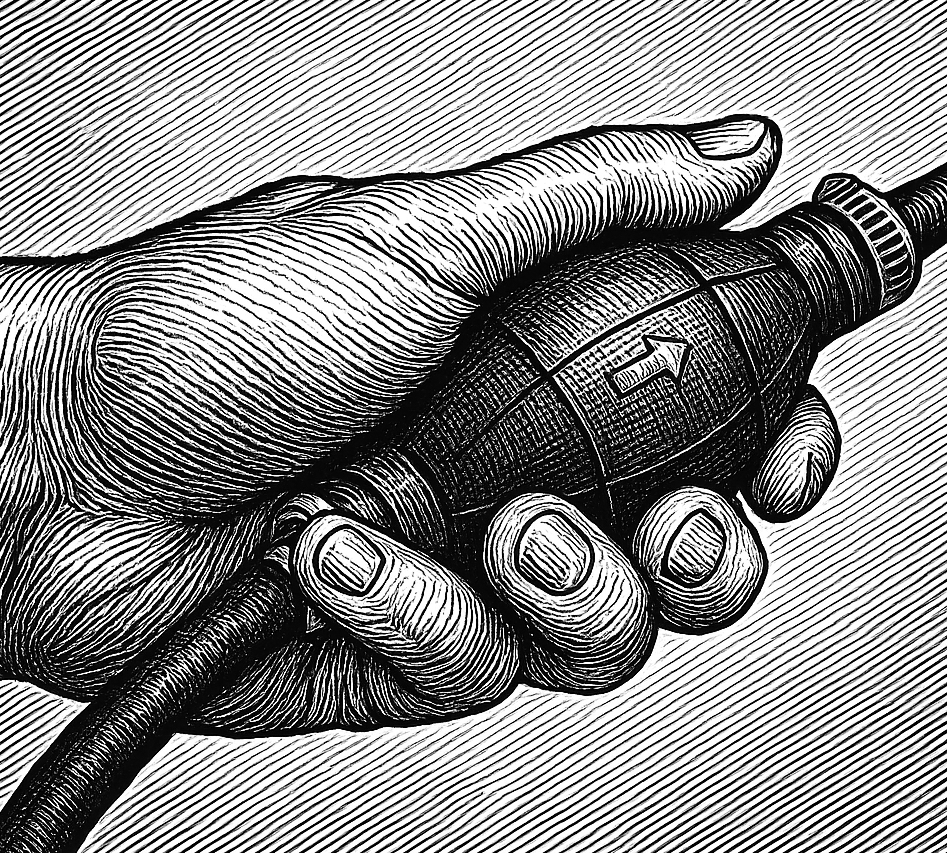
\includegraphics[width=0.5\textwidth]{31_pardon}
	\caption{\small\textit{...где моя, пардон...}}
	%\end{figure}
\end{wrapfigure}раз зажал и разжал грушу, отчего клапан в ней издал чавкающе\sdash булькающий хлюпающий звук.

\diagdash Ы-ы-ы! 

\diagdash Ну как\sdash то так, парни!\mdash Адмирал ещё раз проверил берег на~предмет забытых вещей и велел всем садиться в~байды.\mdash Пока мы собой и байдарочными юбками не~закроем проёмы, байды так и будет непрерывно заливать дождём! Стартуем!

Команда уселась на свои места и закрыла юбки, натянув их на фартук и герметизировав, таким образом, себя от~дождя. Для этого пришлось помучиться\mdash пластиковые трубки, вшитые в фартук, видимо где\sdash то разошлись, а~юбки на~это не~были рассчитаны. 

Наконец отчалили. Адмирал вывел за~борт шланг, подсоединённый к~груше, и~начал откачивать воду из~трюма:

\diagdash Чавк\sdash чавк! Чавк\sdash чавк! Чавк\sdash чавк!

\diagdash Ы-ы-ы!

\diagdash Очень смешно!\mdash укоризненно изрёк Адмирал.

\diagdash Ы-ы-ы! Дай потом нам, у нас тоже воды по~кильсон!\mdash Замполит обошёл адмиральскую байду.

На воду они встали только около полудня, но Адмирал не особо переживал по поводу позднего выхода. Он~вообще решил, ещё в первый день сплава, что постарается как можно меньше переживать в этом походе и как можно больше всё пускать на~самотёк\mdash это не всегда у него получалось, но~всё~же в этом сплаве они паковались довольно расслабленно.

Они потихоньку правили по~Линдозеру в Суну, параллельно откачивая воду из трюмов. Справа на~мысу, где~заканчивалось озеро и~начиналась уже река, ребята увидели хорошую стоянку с большим песчаным пляжем:

\diagdash И чего сюда не пошли позавчера?\mdash спросил Серёга.

\diagdash Не знаю, спроси у Адмирала.\mdash отозвался Замполит.

\diagdash Так занято же! Вон палатки в глубине стоят. И~позавчера стояли. Да и хотелось на острове постоять$\ldots$ \mdash признал Адмирал.\mdash На тебе грушу, я откачался!\mdash он~передал Серёге приспособу.

\diagdash Чавк\sdash чавк! Чавк\sdash чавк! Чавк\sdash чавк!\mdash доносилось теперь с замполитовой байды.

Проходя занятую байдарочниками стоянку, Адмирал увидел там трёх\sdash четырёх$\ldots$ детей! И если когда позавчера эскадра обходила мыс на~острове, те ребятишки не~произвели на Адмирала никакого впечатления, потому что плавсредство там было\mdash моторка, то тут это были дети байдарочников. У Адмирала сразу отлегло и стало как\sdash то светло и~хорошо на душе, хотя погодные условия этому совсем не~способствовали\mdash он окончательно понял, что ничего особо страшного от~этой реки второй категории ждать не~придётся. <<Если здесь с~детьми ходят, то мы\sdash то уж точно выдюжим этот маршрут>>,\mdash подумал Адмирал и~подналёг на весло.

Вода была, без преувеличения, везде: в озере, по~которому они стремительно приближались к Суне и~активной части маршрута, в небесах, откуда их обильно поливало потоками, в байдарках, откуда сплавщики, яростно <<чавкая>> грушей, её откачивали. Вскоре они вошли в~реку, и~по левому берегу сразу началась деревня Линдозеро, правда выглядела она какой\sdash то заброшенной. На берегу была табличка с~телефоном турбазы:

\diagdash А чойта мы в гостишку не приплыли?\mdash угорал Замполит.

\diagdash Ага, крова-а-ать, ко-о-офэ с булочкой, да?\mdash поддержал, угорая, Паша.

\diagdash Потому что имел я видеть в своём отпуске вокруг себя каких\sdash то людей, кроме своей бравой команды!!!\mdash внезапно чуть не взорвался Адмирал.\mdash Кстати кофе молотый у меня где\sdash то есть запасец, сварим завтра, обещаю. Так, парни, впереди гряда островов, идём посередине!\mdash проинструктировал он эскадру.

Островки они вскоре миновали, оставив деревню по~левому борту, и стали подходить к огроменному, метров на~150, старому деревянному мосту через Суну. Мост, когда\sdash то бывший, видимо, автомобильным, безнадёжно обветшал. Вместо каких\sdash то пролётов лежало всего пару досок\mdash местным из деревни ходить в~лес~на~другом~берегу.

Пока они приближались к мосту, особо не гребя, дождик как\sdash то поутих. Адмирал спросил:

\diagdash А чё, парни, деревня же. Связь есть?

Серега, Киря и Руслан полезли проверять:

\diagdash Если чё не загрузил вчера\mdash давай щас,\mdash обратился Адмирал к Замполиту,\mdash а то скоро порог.

\diagdash Описание всё загружено, полностью$\ldots$\mdash Замполит высоко поднимал весло, отрабатывая утренний протеин.

{
%\begin{wrapfigure}[20]{c}{1.0\textwidth}
\setlength{\belowcaptionskip}{0.1mm}
\begin{figure}[h]
	\centering
	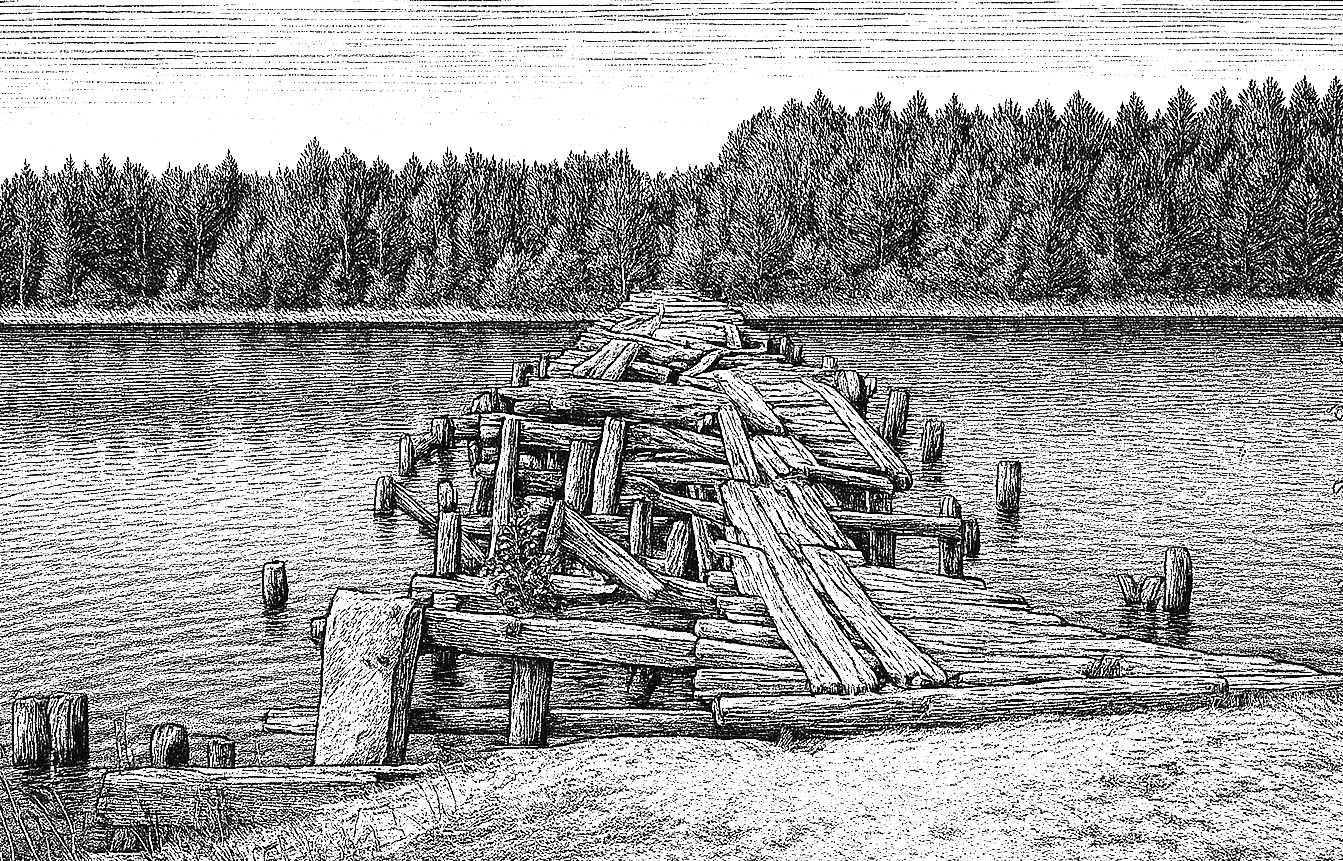
\includegraphics[width=1.0\textwidth]{32_1_bridge}
	\caption{\small\textit{...Вместо каких\sdash то пролётов лежало всего пару досок...}}
\end{figure}
%\end{wrapfigure}

Эскадра вплотную приблизилась к~мосту, облачность стала не такой угрюмой, чуть посветлело, дождь стал совсем редким, как редкая водяная пыль, скорее. 
}

\diagdash Шурик!\mdash Киря упахивался веслом.

\diagdash А?

\diagdash В каком пролёте пойдём?

\diagdash Да давай в центральном! Дай, я первый пойду.\mdash Адмирал вырулил в середину пролёта и сказал своему экипажу не грести\mdash они плавно по инерции медленно приближались к опорам моста. 

\diagdash Шурик, аккуратно!\mdash Замполит заходил следом.

Адмирал, оттабанив, почти полностью погасил скорость, и они шли по течению, поскольку он~перестраховывался от всякой гадости, которая по~обыкновению может лежать или перед мостом, или под~ним\mdash брёвна всякие с гвоздями, балки и прочая ерунда. К счастью, никакой дряни под мостом не оказалось, и они плавно миновали его, стали набирать ход. Адмирал отметил про себя, что мост очень хлипок, проходим пешком просто на~грани экстрима.

Впереди команда заприметила мужиков на двух надувных моторках\mdash те рыбачили на ходу под правым берегом. Адмирал же с Замполитом правили по левому берегу\mdash так было сказано в описании порога, к которому они неумолимо приближались$\dots$ 

Шум Уйтуженкоски они заслышали уже метров за~четыреста. Адмирал взял ещё левее, под самый берег, чтобы было дальше видно порог, который, следуя изгибу реки вправо, уходил за поворот впереди на полкилометра. Ширина русла была огромна\mdash метров 70 у~начала порога. Костяк команды, привыкший к относительно узким и спокойным речушкам вепсовской возвышенности, был маленько в шоке\mdash всё широченное русло Суны, насколько хватало взора, бурлило валами с~белой пеной и барашками. Сплошная шумящая и гремящая каша порога устремлялась вдаль за поворот.

\diagdash Пристаём к левому берегу!\mdash отдал команду Адмирал.\mdash Аккуратно только заходим, там камни!

\diagdash Охренеть каша белая!\mdash экипажи прибалдели.

Команда, подзатащив байдарки на прибрежные валуны у мелководья левого берега и оставив их так, прошла пешком чуть дальше, насколько позволяли камни:

%\begin{wrapfigure}[20]{c}{1.0\textwidth}
\begin{figure}[h]
	\centering
	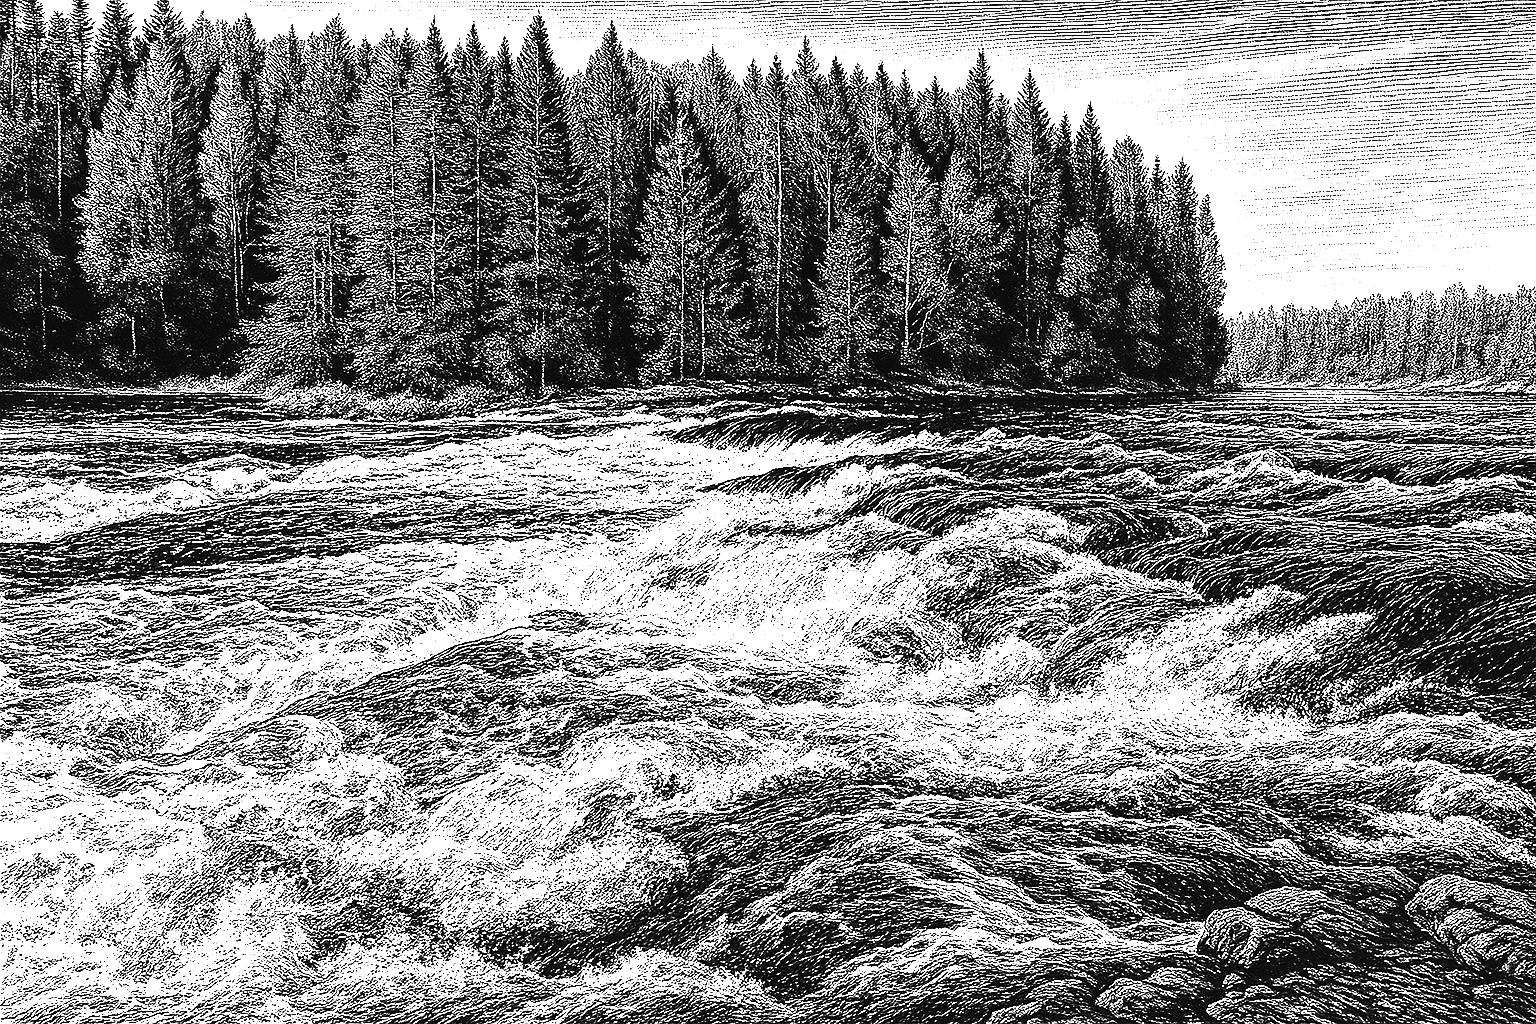
\includegraphics[width=1.0\textwidth]{33_1_porog}
	\caption{\small\textit{...Шум Уйтуженкоски...}}
\end{figure}
%\end{wrapfigure}

\diagdash Охренеть!!!

\diagdash Ты видишь куда тут идти?!?!

\diagdash Валы по метру!!!

\diagdash Ёпрст!!!

Они стояли и чесали затылки, рассматривая бурлящую и кипящую, словно в каком\sdash то колдовстве реку. Действительно, ни на секунду не прекращающееся холодное кипение было похоже на что\sdash то такое нереальное, неестественное, чего не может быть в сознании человека, выросшего на спокойных размеренных реках средней полосы~России.

\diagdash Ну, надо идти. Киря, доставай и читай описание порога!\mdash очнулся от завораживающего созерцания~Адмирал.

\diagdash Ага! Так$\ldots$ <<На входе под левым берегом шивера с~бурным течением>>. Ну вон она, походу!\mdash он неуверенно показал куда\sdash то вперёд.

\diagdash Ну типа. Дальше давай!

\diagdash <<Далее надо переходить под правый берег>>. Хм-м-м!

\diagdash Логично, парни, смотрите какие валы слева! Там~до~метра, походу!\mdash Адмирал показал вперёд чуть левее, примерно на середину того, что было перед их~глазами.

\diagdash Охренеть, охренеть!\mdash только и повторял Замполит. Серёга и Руслан молча стояли, смотрели на бурлящую пену, а Паша с Адмиралом, стоя на камне, прикидывали как и что.

\diagdash Кирь, давай читай, хар{\'о}ш рефлексировать!

\diagdash Ага. <<Ближе к~выходу поток стесняется остатками плотины и отмелью слева, образуя крутую горку со стоячими валами. В низкую воду в~струе появляются два опасных обливняка, хорошо заметных по пенным гребням за ними>>$\ldots$

\diagdash Хорошая новость\mdash низкая вода это не про нас\mdash смотрите на прибрежные камни! Когда вода спадает, на них такие полосочки образуются, а сейчас ничего такого нет.\mdash заключил, воодушевляя всех, Адмирал.

\diagdash Да, походу ты прав$\ldots$

\diagdash Короче, парни! Паш, смотри тоже сюда.\mdash Адмирал встал повыше на камни и стал размахивать руками.\mdash Заходим ровно по центру сначала\mdash тут всё равно как идти, похоже. Дальше, как и сказано в описании, прижимаемся к~правому берегу, обходя вон ту жесть,\mdash он показал на~самые высокие валы в пороге слева,\mdash а потом как пойдёт, но я подозреваю, что лучше правого берега держаться.

\diagdash Шурик, ты уверен?\mdash Серёга грустновато смотрел в~порог.

\diagdash А есть ещё варианты? Погнали! Замполит, убирай мобильник, чтоб не утопить, и врубай рацию. Как пройдём, я~выйду на связь!\mdash обернувшись к~экипажам, он махнул рукой.\mdash Надеваем спасы! По коням, парни!

Хоть Адмирал и хорохорился, на душе у него были такие терзания, что просто не передать. Он притух от~уходящего в неизвестность белого бурлящего потока, но в то же время вспомнил про тех байдарочников с детьми\mdash это немного придало ему сил. Его экипаж уселся в~байду и стал отчаливать. Адмирал был, как ему казалось, на~эмоциональном пике, хотя основный пик ещё был впереди:

\diagdash Так, отходим выше по течению, разворачиваемся, выравниваемся по руслу и ровненько заходим на <<язык>>.\mdash Адмирал застегнул байдарочную юбку, герметизировав себя в фартуке.

\diagdash Куда заходим?\mdash экипаж тоже копошился с~байдарочными юбками.

\diagdash Ну на <<язык>>\mdash вон в первой ступени порога читается такой треугольничек тёмной воды на сливе\mdash там должно быть поглубже.\mdash Адмирал упёр весло в~фартук и~фальшборта, усаживаясь повыше.\mdash Застёжки спасжилетов проверьте! Начали!

\diagdash Сань, да погоди ты, я юбку не закрыл!\mdash бросил Пашка.

\diagdash А?\mdash не расслышал на корме Адмирал.

\diagdash Погоди, говорю!!!

\diagdash Мы заходим!!!

\diagdash Ё-ё-ё!!!

Адмирал выровнял курс и, сам не зная почему, поднёc два прямых перста правой руки ко лбу:

\diagdash {\'{O}}дин, всеотец, будь с нами$\ldots$\mdash почти беззвучно прошептал он, а потом заорал:\mdash {\large ВПЕРЁ-Ё-ЁД!!!!!!!!!!!!!!}

Они зашли на <<язык>> и нырнули в порог\mdash стихия моментально разогнала их байдарку, они успешно миновали вход. Порог стремительно увлекал их судёнышко в самую гущу событий, в бурлящие и клокочущие валы:

\diagdash {\large ЛЕВЫМ!!! ЛЕВЫМ!!!}\mdash заорал Адмирал, когда волны кидали их корабль, как щепку, а беспорядочное течение и завихрения потока стали заворачивать их левее, где были огроменные стоячие валы.\mdash {\large УПЁРЛИСЬ} 
\makebox[\linewidth][s]{\noindent {\large ЖЁСТКО ПО~ЛЕВОМУ!}\mdash продолжал орать Адмирал,}
%ЖЁСТКО ПО~ЛЕВОМУ!!!}\mdash продолжал орать Адмирал,

%\begin{wrapfigure}[20]{c}{1.0\textwidth}
\begin{figure}[h]
	\centering
	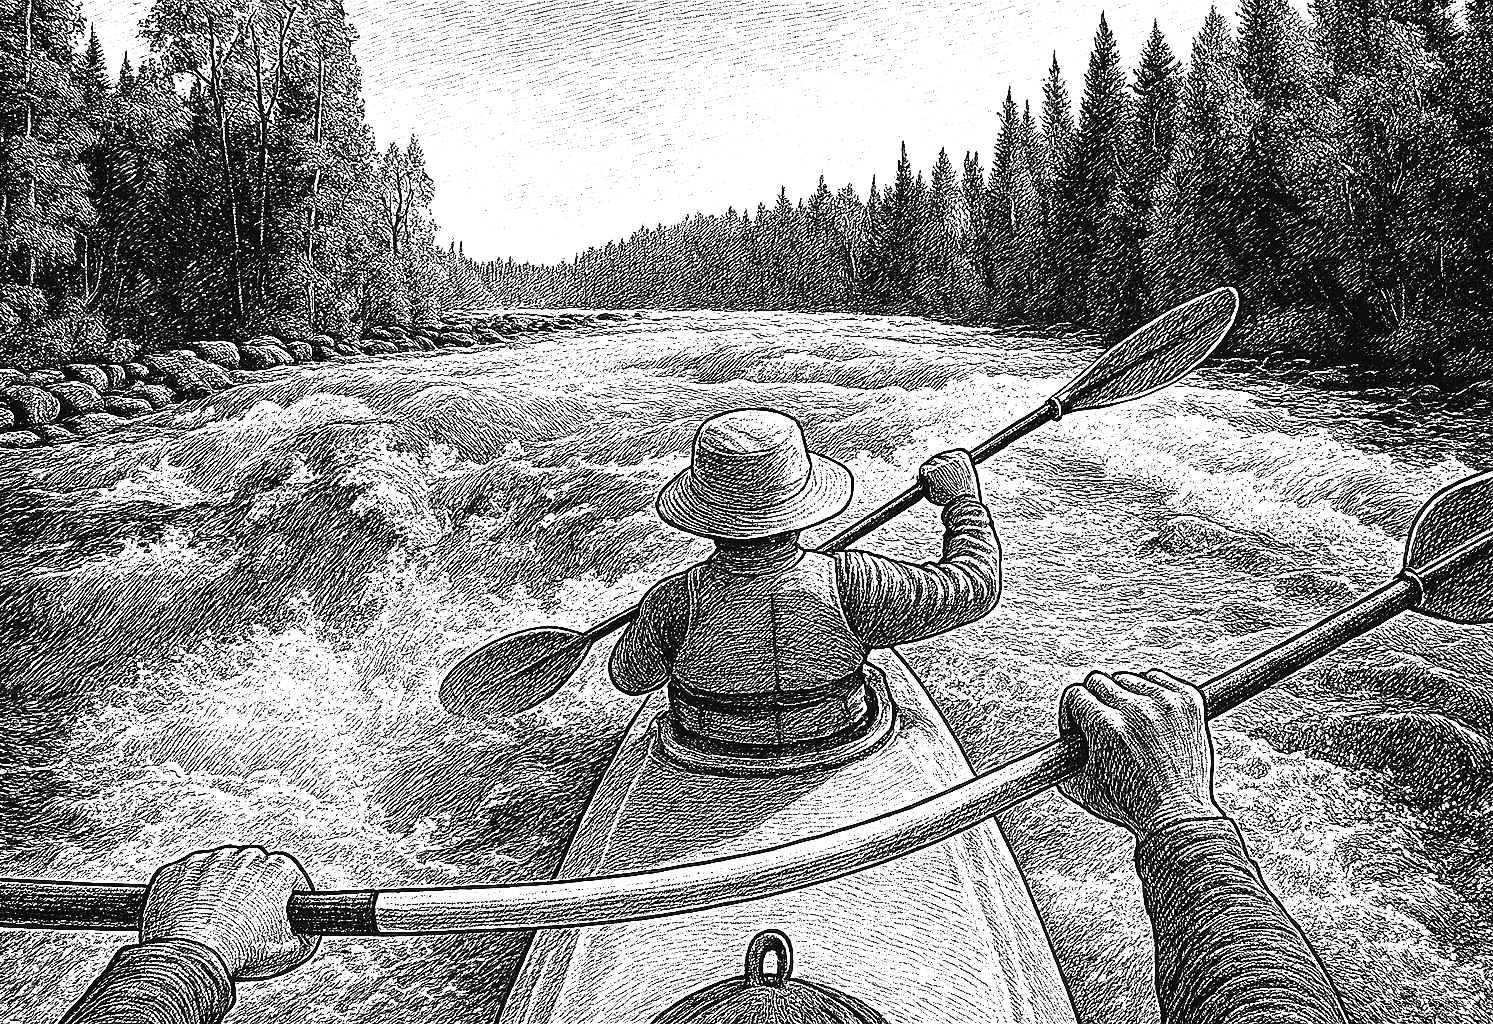
\includegraphics[width=1.0\textwidth]{34_1_shturm}
	\caption{\small\textit{...УПЁРЛИСЬ ЖЁСТКО ПО~ЛЕВОМУ!..}}
\end{figure}
%\end{wrapfigure}

\noindent перекрикивая шум порога. Парни молниеносно отгреблись, а он сильно затабанил слева, вновь выровняв курс и встав ровно перпендикулярно валам. 

\diagdash {\large ПОЛНЫЙ НАХОД!!!}\mdash они пошли пробивать огроменные валы, нараставшие один за другим впереди: один\mdash БАМ!!!\mdash второй\mdash БАМ!!!!!!\mdash третий\mdash БАМ!!!!!!!!!

Волны окатывали их по полной, не щадя! Нос байдарки зарывался в~валы так, что Адмирал чувствовал, как кровь стынет у него в жилах! Холодная вода порога окатывала и Пашку, сидящего впереди, и Руслана, и~даже успевала докатиться до Адмирала на корме\mdash залило в юбку, а уж с вёсел экипажа ему и~вовсе летели брызги прямо в глаза. Экипаж чётко отрабатывал все адмиральские команды, которые приходилось орать, перекрикивая шум, грохот даже, воды. Они ровнёхонько встречали вал за~валом, продвигаясь вперёд. Наконец, посреди порога, уже на~cамом повороте, максимальной точке, которую они смогли просмотреть перед началом штурма, вода внезапно чуть подуспокоилась, можно было подрасслабиться. Адмирала захлестнула просто такая эйфория, какую он, пожалуй, никогда и ни от чего в своей жизни не испытывал. Это было чувство выжившего, чувство превосходства над~стихией, восторженность от преодоления и порога, и самого себя, своих страхов и неуверенностей, это~было то чувство, тот эмоциональный подъём, за~которым они все без исключения оказались тут. 

Их стало немного разворачивать к правому берегу:

\diagdash {\large Э!!! САНЯ!!!}\mdash заорал спереди Пашка.

Адмирал, очнувшись, воспрял и жёстко затабанил слева, они вновь пошли ровно на валы\mdash начиналась вторая ступень порога:

\diagdash Готовимся, парни!!!

\diagdash Ага!!! Ровненько!

%\renewcommand*{\thefootnote}{\arabic{footnote}}
\renewcommand*{\thefootnote}{\fnsymbol{footnote}}
\setcounter{footnote}{0}
Секунда и новые валы окатили их, байдарка ходила ходуном, дифферент\footnote{Дифферент (от лат. differens, differentis\mdash разница)\mdash наклон судна в продольной плоскости.} на нос и корму достигал каких\sdash то жутких значений. Адмирал старался править так, чтобы заходить к новому валу максимально перпендикулярно, исключая опасность боковой качки и оверкиля, врезаясь в~бурлящую воду носом. Чувство эйфории не проходило\mdash они успешно проходили остаток порога. Впереди у правого берега была гряда торчащих из воды камней, а у левого\mdash мель и брёвна. Посередине, S\sdash образным изгибом влево и тут же вправо, шла основная струя. Адмирал понял, что это, возможно, и есть остатки какой\sdash то там плотины из описания, и им туда\mdash пора было выходить из\sdash под правого берега ближе к середине русла, чтобы не напороться на камни:

\diagdash {\large ПРАВЫЙ НАХОД!}\mdash заорал он, а сам слегка оттабанил слева и они идеально вошли в стремнину. Далее он оттабанил справа, и парни, легко пройдя уже не~такие высокие, как ранее, валы в конце порога, вышли на~спокойную воду, по которой дальше плыла взбитая стихией пена. Адмирал отметил про себя, что парни оказались очень удачным экипажем\mdash опытный передний гребец и новичок, схватывающий всё на лету\mdash ни~разу, ни~сейчас, ни~на~Нурмисе, никто из них не перепутал куда надо грести, следуя адмиральским указаниям, и они идеально, или почти идеально, проходили препятствия в~русле.

\diagdash {\large ПРОШЛИ!!!}\mdash кричали они.

\diagdash Руслан, Паш, как вы?\mdash Адмирал правил к~островочку посередине заводи после порога.

\diagdash Я те орал: <<Погоди!>>, а ты попёрся!!!\mdash Пашка обернулся.\mdash Я ж юбку не до конца закрыл!!!

\diagdash Налило?

\diagdash Да я весь мокрый! Все штаны!!!

\diagdash Ё-ё-ё!!!

\diagdash Да чё теперь!!!

Адмирал развернул байду против течения и подошёл к~острову посреди русла, стал промерять веслом глубину:

\diagdash Парни, тут гл{\'ы}боко! Не вылезешь особо, давай ещё чуть поближе, за траву прибрежную хватайтесь!

Они подсадили нос байды на гладкие валуны, открыли байдарочные юбки и поглядели на днище:

\diagdash Твою ж!!! Воды по щиколотку!!!\mdash Адмирал прибалдел от увиденного.\mdash Откуда?!?!

\diagdash А я тебе о чём?!?!?! Залило капитально!!!\mdash Пашка вымок и, естественно, негодовал.
 
\diagdash Руслан, а ты как?

\diagdash Ну, через юбку не натекло, сверху только брызгами намочило нехило так$\ldots$

\diagdash Блин$\ldots$ Извиняй, Паш! Я не понял, что ты не~закрылся!\mdash Адмиралу стало неловко перед товарищем.\mdash Походу, это всё через твою юбку нахлестало.

\diagdash Ну а как ещё? Ладно, забей$\ldots$ Всё равно вымокнем$\ldots$

Адмирал достал рацию и вышел в эфир:

\diagdash Киря, мы прошли, вообще круто!!! Просто огонь!!! Короче, входите ровненько, как мы, а дальше идите чуть левее самых высоких гребней валов у правого берега. В~середине вода чуть поуспокоится перед второй ступенью порога. Как понял? Приём!

\diagdash Шурик$\ldots$ Там есть вторая ступень? Приём!

\diagdash Да, мы же читали! Она проще первой, там будет такой S\sdash образный поворотик, надо уходить из\sdash под правого берега ближе к центру. В~целом, ничего страшного, везде глубоко. Давайте, жмите! Закрывайтесь только юбками хорошо, нам по щиколотку нахлестало воды! Приём.

\diagdash Понял, ждите$\ldots$ Мы потихонечку начинаем.\mdash голос у Замполита был, конечно, так себе. <<Очкует>>,\mdash подумал Адмирал и отложил рацию.

\diagdash Сань, надо отчерпываться$\ldots$ \mdash Пашка возился спереди, пытаясь вылезти.

\diagdash Тут фиг вылезешь, да и место не располагает. Блин, дрочилка забилась, не фурычит!\mdash Адмирал попытался прочистить грушу, но не получилось\mdash видимо клапан заело грязью.\mdash Как отчерпываться\sdash то?

\diagdash Да этой грушей мы вечность выкачивать будем!

\diagdash Ну да$\ldots$ \mdash Адмирал хотел достать свою кружечку, чтобы отчерпаться ей, но вспомнил, что отчего\sdash то переложил её с утра в вещмешок из кармана штормовки. А лезть в~вещмешки на плаву было идеей так себе, поэтому в итоге он решил отчерпываться крышкой термоса, который был под рукой. Занятие было чертовски скучным, монотонным и требующим отрешения, Адмирал сидел у себя на корме и~потихоньку осушал трюм.

Вид на бурлящую порогом реку уходил вдаль вверх по~течению, ребята то и дело пристально вглядывались в~белую пену, силясь увидеть второй экипаж:

\diagdash Что\sdash то не идут! Может вызвать их по рации?\mdash протянул Адмирал, отчерпываясь.\mdash Разброд и шатание!

\diagdash Если бы чё\sdash нить случилось, уже бы вещи поплыли$\ldots$ \mdash отжигал Паша.\mdash Так что не кипишуй, черпайся!

\diagdash Тьфу ты!

\diagdash Ы-ы-ы!

Адмиралу наскучило черпаться, хотелось перекурить после прохождения порога. Он передал крышку от термоса Руслану и тот продолжил дело. Адмирал же откинулся назад, вытащил портсигар, уселся поудобнее, насколько это было возможно, и задымил.

\diagdash Идут!\mdash Пашка увидал второй экипаж, показавшийся из\sdash за поворота. 

\diagdash Первую ступень прошли, черти. Дальше\mdash проще.\mdash Адмирал, щурясь, вглядывался в белеющую кашу порога, следя за~замполитовой байдой, то и дело исчезавшей за~высокими валами.% и вновь появлявшейся, пробив очередную водную стену.

<<Пора, пора! Надо выходить из\sdash под правого берега, на стремнину! Ну же!>>\mdash думал Адмирал, смотря на то, как замполитовский экипаж ныряет в валы, пробивая их. Наконец, Киря, видимо, осознал стратегию прохождения и круто заложил к центру реки\mdash прямо на валы в~S\sdash образной части последней ступени порога. Дифферент на~нос и корму был нехилый\mdash теперь адмиральский экипаж имел возможность посмотреть, как красиво и одновременно страшно это выглядит со стороны: нос байдарки зарывался в белую пену, вода заливала носового гребца так, что только юбка и фартук были спасением. Киря и Серёга лопатили вёслами так, что дюралевые лопасти только и сверкали. Адмирал, стараясь не нервничать, сам того не заметил, как наблюдая за их прохождением, доканчивал вторую папиросу.

\diagdash {\Large ПРОШЛИ-И-И!!! А-А-А!!!}\mdash орал во всё горло замполитовский экипаж.

\diagdash {\Large Й-Й-Й-О-О-О-У-У-У!!!}\mdash приветствовал их адмиральский экипаж.

\diagdash Налило?\mdash Адмирал потушил папиросу.

\diagdash Да охренеть!!! Надо отчерпываться капитально, кильсон весь в воде!\mdash Киря разворачивался и заходил параллельно к адмиральской байдарке, эмоции так и били ключом.\mdash Шурик, дай закурить!!!

\diagdash Ы-ы-ы!!!

\diagdash Вот те и <<Ы>>!

\diagdash Забей! Живы, здоровы, эмоций через край! Я~просто в эйфории!!!\mdash Адмирал вытащил портсигар,\mdash С приветом от пульмонолога.\mdash и протянул Замполиту папироску.\mdash Главное там засада какая\mdash после первой ступени вроде как вода подуспокоилась,\mdash он жарко жестикулировал руками,\mdash и я на связь хотел выйти, да пока доставал рацейку, уже вторая ступень на подходе, и Пашка орёт, мол, давай рули!!!

\diagdash Да ваще жесть!!!\mdash Замполит прикурил и~затянулся.\mdash Я рулю, а Серёга там лопатит, лопатит, ух ё!

\diagdash Ну да, там посередине как передышка была относительная,\mdash согласился Серёга,\mdash а потом опять жесткач!!!

\diagdash Кайфец полный!

\diagdash А то!

\diagdash Ради этого, собстно, мы сюда и припёрлись!!!

\diagdash И не говори$\ldots$ Ладно, надо отчерпываться!

\diagdash Дай кружечку, у нас воды там ё\sdash моё!

\diagdash На!\mdash Адмирал протянул тому крышку о термоса.

После того, как они осушили, как могли, свои трюмы, ребята отчалили от островочка и стали править дальше к~следующему порогу, который... отсутствовал. При подходе к~точке, обозначенной на карте и в навигаторе, команда не обнаружила ничего, что могло хотя бы отдалённо напоминать порог. Никакой стремнины не было и в помине.

\diagdash Шурик, кто украл порог?\mdash осведомился Замполит. 

\diagdash Хрен знает! Но место явно то, что на карте\mdash и~характер берегов совпадает, и GPS нас тут показывает.\mdash Адмирал не особо удивился, он читал в отчётах по маршруту, что на старой карте есть <<лишний>> порог.\mdash Может воды чересчур много? Хотя навряд ли, всё равно бы чего\sdash нибудь да~бурлило всё равно$\ldots$

Последовало протяжённое правое искривление русла, и~прямо перед сплавщиками начала нарастать безымянная гора, у которой река делала крутой, чуть не на 90 градусов, правый~поворот. Ребята увидали на крутом правом берегу, где откосы были примерно 30\thinspace\nobreakdash---\thinspace 40 градусов, стоянку двух каякеров\mdash парня и~девушки. Те были в~гидрокостюмах, на пластиковом двухместном каяке, и~уже были готовы отчаливать. Команды поприветствовали друг друга, и~Адмирал с~Замполитом стали заходить в~поворот, из\sdash за которого стал слышен шум порога.

\diagdash В описании не было про него ничего?\mdash уточнил Серёга.

\diagdash Не-а!\mdash ответил Адмирал,\mdash Значит там и~просматривать особо нечего, штурмуем сходу! И\sdash и\sdash и\sdash ха!\mdash и~первым устремился в порог.

Второй Безымянный, как прозвал его про себя Адмирал, они просквозили вообще легко\mdash путь прохождения шиверы читался хорошо, никакой жести особо не~было, валы были уже не~такие огромные как в~Уйтуженкоски, но тоже достаточно сильные и мощные.

\diagdash Е\sdash е\sdash е!!!

\diagdash Ещё один прошли!!!

\diagdash У\sdash ху\sdash ху!!!\mdash эйфория от катания по валам была у~пацанов мощнейшая. Они радовались преодолению стихии и просто кайфовали от катания по волнам и валам\mdash это не~на~шутку щекотало нервы, принося массу адреналина.

Река плавно повернула с юго\sdash востока на северо\sdash восток и начала приближаться к порогу Шильмятойкоски. Адмиральский экипаж шёл первым, Замполит не отставал. Вскоре парни заметили на правом берегу стоянку большой группы\mdash те~то~ли~дневали, то~ли собирались вставать на~воду\mdash было не разобрать, а~останавливаться и~трепаться не~хотелось.

\diagdash Шурик, мож это те, которых мы перед Нурмисом сделали на озере?\mdash Замполит поровнялся с адмиральской трёшкой.

\diagdash Может, почему нет?\mdash отозвался тот.

\diagdash Хорошо бы отдохнуть чутка?

\diagdash Порог скоро$\ldots$ Ну давай чутка почилим, у левого берега.

Парни прибились к прибрежным зарослям и вытащили термосы с чаем, чуть отдохнули от гребли.

\diagdash Чё дальше у нас по плану?\mdash спросил Серёга.

\diagdash Порог Шильмятойкоски. Тащ Замполит, доставай описание.\mdash Адмиралу не терпелось идти дальше.

\diagdash Угу!\mdash Замполит открыл гермочехол и~вытащил мобильник.\mdash Та\sdash а\sdash ак, что тут у нас? Шильмятойкоски. <<Порог оленьих загонов. Это пятисотметровая шивера с~правым поворотом в конце и высокими прямыми валами в главной струе>>, хм\sdash м\sdash м, дальше бла\sdash бла\sdash бла, а вот это интересно: <<После поворота в~струе мощная <<бочка>> за~плитой, поэтому на повороте надо прижиматься к гряде камней, идущей от правого берега. Справа перед порогом есть хорошая стоянка>>.\mdash Замполит оторвался от телефона.\mdash <<Бочка>>, мать её!

\diagdash Ну, <<хорошая стоянка>>, я так понимаю, занята вон теми деятелями, которых мы прошли недавно.\mdash резонно заметил Серёга.

\diagdash Ага$\ldots$\mdash согласился Адмирал.\mdash$\ldots$<<Бочка>> за~плитой, прижиматься там рекомендуют правее. Верно,~Кирь?

\diagdash Да вродь как. Ну сам смотри: <<$\ldots$на повороте надо прижиматься к гряде камней, идущей от правого берега$\ldots$>>\mdash правее, но это не точно.

Тут команду, попивающую чай под берегом, обогнали те парень с девушкой в гидрокостюмах. Пара пожелала сплавщикам хорошего прохождения и скрылась впереди на~своём красном пластиковом каяке. Адмирал посмотрел им вслед, допил чай, убрал термос и закрыл юбку:

\diagdash Короче, погнали уже! Все готовы?

\diagdash Так точно, тащ Адмирал! Только ты первый давай, а~мы\mdash за тобой!\mdash Замполит убирал мобильник в герму.

\diagdash Ы-ы-ы! Ну давайте, готовьтесь потихоньку, мы начинаем. Как пройдём порог\mdash попробуем причалить где\sdash нибудь и выйти на связь по рации. Кирь, рацейку проверь, мы погнали!

\diagdash Давай! Ни пуха!

\diagdash К чёрту!

Адмиральский экипаж оттолкнулся от берега и стал выходить на середину русла:

\diagdash Так, парни. Спокойненько, не торопимся. Юбки на этот раз все закрываем нормально. Не гребите, я пока повыруливаю, а вы закрывайтесь как следует, герметизируйтесь.\mdash вещал Адмирал с кормы, а самого терзали мысли о <<бочке>>. Он много раз читал об этой страшной штуке в туристических отчётах и просмотрел не~одно видео при подготовке к походу, но всё равно чувствовал себя неуверенно сейчас. <<Прижиматься правее, прижиматься правее на~повороте>>,\mdash мелькало в его голове,\mdash<<ох уж эта <<бочка>> за <<плитой>>$\ldots$ Знать бы ещё что за плита$\ldots$ Ладно, спокойно, потихонечку>>.

\diagdash Ну вроде готов$\ldots$\mdash бросил Пашка с носа.

\diagdash Руслан?

\diagdash Готов!

\diagdash Поехали!\mdash адмиральский экипаж подналёг на весла, последовал изгиб русла влево и сразу же на правом повороте и они вошли в порог.

\diagdash {\large ПОЛНЫЙ НАХОД!!!}\mdash проорал Адмирал, а сам попытался хоть на миллиметрик высунуться повыше, карауля проклятую <<бочку>>.\mdash {\large НОРМАС, ТАК ДЕРЖИМ!}\mdash они стремительно пошли сквозь пенные валы, выбирая путь поспокойнее, для чего Адмирал подруливал, то табаня, то~усиливая наход экипажа. 

\diagdash {\large САНЯ, ГРЯДА!}\mdash проорал на носу Пашка.

\diagdash {\large ДА!}\mdash Адмирал тоже, как, видимо, и Пашка, почувствовал, что их начинает утягивать затяжным левым поворотом порога и сносить на эту самую каменную гряду. 

Повсюду вода кипела холодными брызгами, заливая их юбки и фартук. Примерно в середине поворота Адмирал решил круче взять влево, чтобы на выходе обойти стоячие валы, которые стали им отчётливо видны.\mdash {\large УПЁРЛИСЬ ЖЁСТКО!!!}\mdash проорал он экипажу, а сам, поймав момент, затабанил по правому борту, переложив курс, следуя изгибу русла и обходя бурлящую кашу. 

Они обходили каменную гряду по правому борту и их взору открылся выход из порога после довольно протяжённого и очень плавного спуска: 

\diagdash {\large НЕ ГРЕБЁМ, РОВНЕНЬКО!}\mdash он вырулил уже сам, помощь экипажа не требовалась.

\diagdash {\large Й-й-й-о-о-о-у-у-у!!!}\mdash их байдарка прошла чуть правее последних пенных барашков и, рассекая пену, взбитую порогом, вышла победительницей из этой схватки со~стихией.\mdash {\large У-у-у-х-х-х-у-у-у!!! Прошли-и-и!!!}\mdash орали они.

\diagdash Как оно, парни?\mdash Адмирал тихонько подгребал, забирая к правому берегу.

\diagdash Ваще-е-е по ка-а-айфу!!!\mdash Руслан, обернувшись, глядел на пологий выход с валами, только что преодолённый~ими.

\diagdash А то, т\'{а}щи м\'{о}тросы! Вы у меня ваще красавцы! Ну,~давайте~к~той гряде с обратной стороны подойдём, подождём Кирю.

Они развернулись под правым берегом против течения и подошли к гряде, Адмирал ювелирно пришвартовался к~валунам. Пашка выпрыгнул на камни и, вытащив чалку, надёжно закрепил её на большом валуне. Потом они ещё подзатащили байду на берег для надёжности и, наконец, смогли окончательно выдохнуть.

\diagdash Класс ваще! И никакой <<бочки>>! Надо фотик взять их пофоткать в пороге, как пойдут! А то без экшн\sdash камеры видосов прохождения так и не сделали, аля\sdash улю!

\diagdash Ты лучше выйди на связь, скажи им, что всё норм?\mdash отряхиваясь, сказал Пашка Адмиралу.

К этому моменту солнце начало пробиваться сквозь облака, облачность рассеялась, показалось голубое небо, погода значительно улучшилась. Утренний дождь воспринимался теперь как нечто давно прошедшее и~не~стоящее внимания. Адмиралу стало безумно хорошо и~приятно, даже каменистая гряда, на которой они высадились, вдруг стала какой\sdash то приветливой в тёплых солнечных лучах. Он сновал по камням и фоткал порог, их~байдарку, экипаж.

\diagdash Да меня\sdash то что снимать? Снимай, вон, порог. И~на~связь лучше выйди!\mdash Пашка в дождевике и~спасжилете выглядел несколько комично, как, впрочем, и все они, и, естественно, был ещё зол на Адмирала за~промокшие в~первом пороге штаны. 

\diagdash Ща, сбацаем.\mdash тот снял дождевик и вытащил рацию из гермы.\mdash Киря, мы прошли, как слышно? Приём!\mdash сказал Адмирал и отпустил тангенту.

А в ответ\mdash тишина$\ldots$ Он снова попытался их вызвать:

\diagdash Киря, Серёга, как слышно меня? Мы прошли нормально! Приём!

А в ответ\mdash тишина$\ldots$

\diagdash Серёга, Кирюха, на связь! Приём!

\diagdash Не слышат$\ldots$\mdash Пашка разминал ноги.

\diagdash С чего бы? Между нами меньше километра!

Адмирал проверил, что в рации стоит полная мощность на передачу и попробовал снова:

\diagdash Серёга, Кирюха, на связь!

А в ответ\mdash тишина$\ldots$

\diagdash Да мать вашу за ногу! Чё делать то?!

\diagdash Чё делать, чё делать, сухари сушить!\mdash передразнил Пашка.\mdash Они начали, небось, уже, и убрали рацию в герму.

\diagdash Так договорились же, что я выйду на связь сперва.

\diagdash Ну-у-у, может их задолбало ждать?

\diagdash Чёрт бы их побрал, никакого порядка, разброд и~шатание!\mdash Адмирал начал вскипать.

\diagdash Да подождём просто их?\mdash вставил было Руслан.

\diagdash Просто, блин!\mdash Адмирал внезапно вспылил и, взяв зеркалку, рацию и весло, пошёл по каменистой гряде против течения, чтобы иметь возможность заглянуть за поворот.

\diagdash Да не парься, никакой жести в пороге не было, щас они придут, ну?\mdash Паша достал трубочку и задымил.

\diagdash Угу! <<Инфаркт микарда, вот такой рубец!!!>>\mdash прокричал, перекрикивая порог, Адмирал, показывая руками величину рубца с косую сажень, и пошёл ещё выше по~течению.

\begin{figure}[h]
	\centering	
	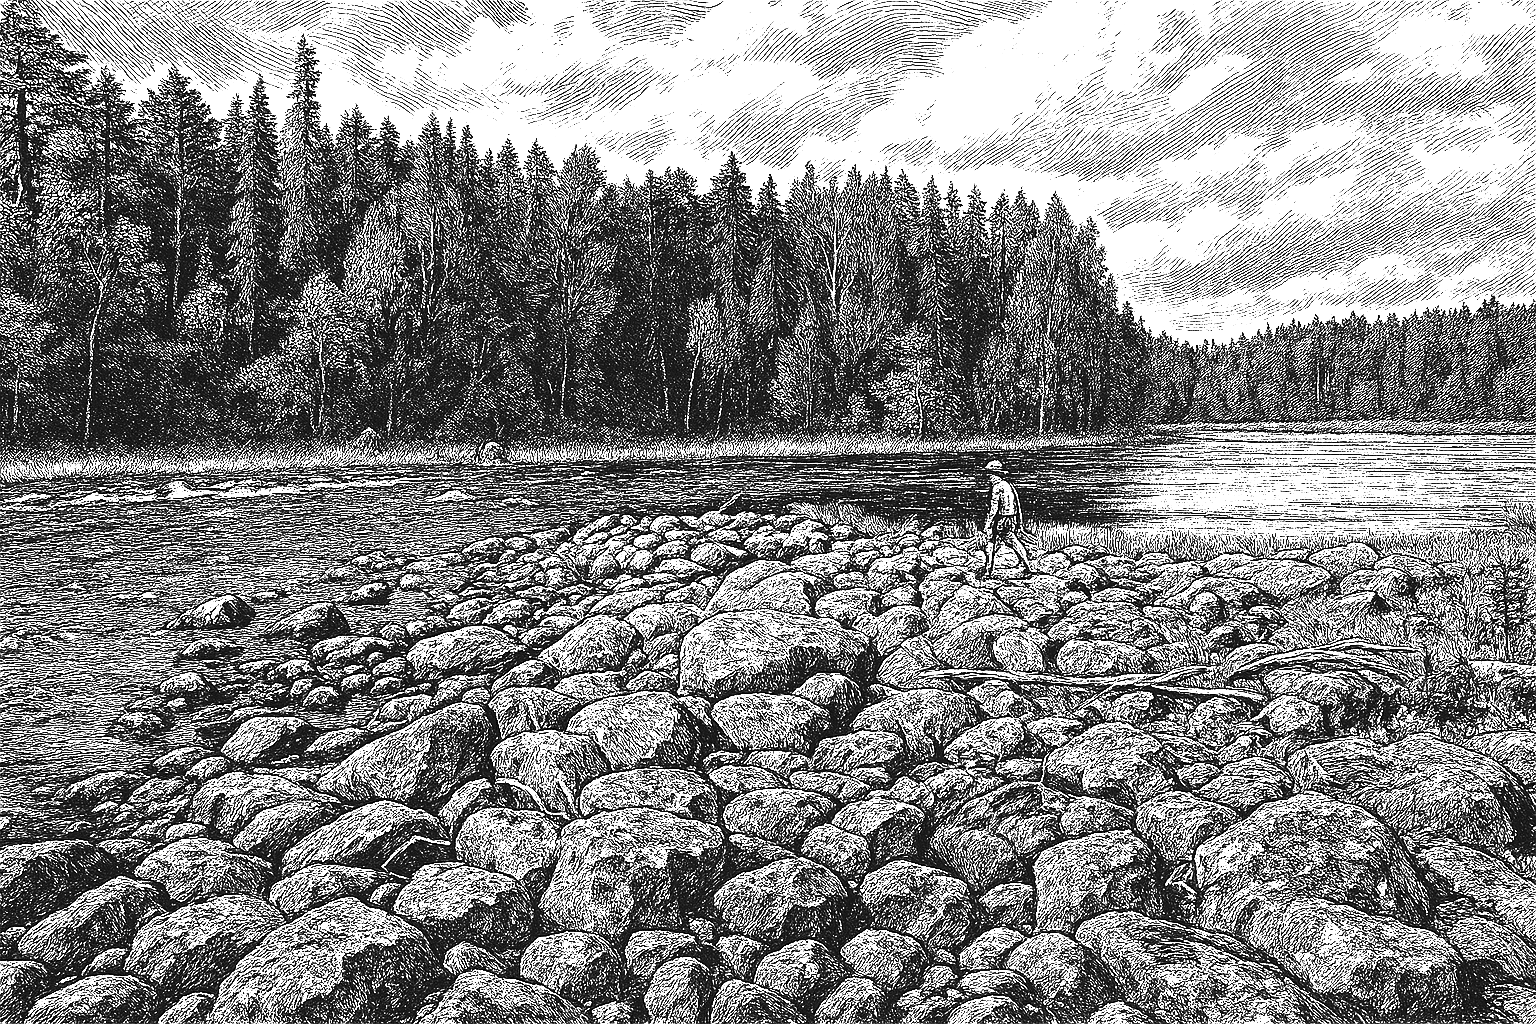
\includegraphics[width=1.0\textwidth]{35_1_otmel}
	\caption{\small\textit{...пошёл по каменистой гряде против течения...}}
\end{figure}

Ему удалось пройти берегом по шатающимся камням почти до~самого начала гряды, а второй экипаж всё не было видно. <<Ну, черти, добавите вы мне седых волос!>>,\mdash шёл он, чертыхаясь на каждом валуне. Наконец, когда дальше идти посуху больше не было никакой возможности, он остановился и стал всматриваться в поворот реки. Тщетно, ни души$\ldots$

\diagdash Серёга, Кирюха, на связь!\mdash неоднократно вызывал он, но рация лишь молчала в ответ. Адмирал глянул на~свои китайские ролексы\mdash было без четверти четыре. <<Так,~ну~на~байдарке идти назад невозможно\mdash придётся её разгрузить тогда и притащить сюда, повыше, на руках, а~потом, упираясь, пытаться перегрести порог, чтобы удрать против течения к ребятам$\ldots$ Ох ты ж ё\sdash моё!>>\mdash он стоял и~размышлял, что ему, как руководителю, стоит предпринять в таком случае. Он прикинул, что торчат они тут с~экипажем на каменистой гряде уже минут 20. <<За это время можно уже было пешком прийти сюда, а их всё нет и~нет! Ну~что~ты~будешь с ними делать! Опять двадцать пять, как на Нурмисе!>>\mdash подумалось ему. 

Ожидание неизвестного тянулось мучительно долго. Наконец, спустя ещё минут десять тягостных раздумий и~безуспешных вызовов по рации, Адмирал увидал свой второй экипаж вдалеке на повороте. Те~шли пешком по берегу в~кустах, такое впечатление, что таща байду на чалке: 

<<Что за хрень?>>\mdash подумалось Адмиралу.\mdash <<Пробились? Но как? Где?>>

Он стал махать им руками. Спустя пару минут они заметили его и тоже помахали в ответ. Ещё немного погодя он увидел, как они сели в байдарку и начали прохождение, отойдя от берега.

\diagdash Ну, черти!\mdash Адмирал был раздосадован ситуацией, но~одновременно рад, что видит товарищей живыми и~невредимыми.

Увлекаемый порогом, экипаж Замполита стал подходить к гряде, а Адмирал, пройдя немного вниз по~течению, встал поудобнее и приготовился заснять на фото и~видео их~прохождение. Наконец, они прошли мимо него:

\diagdash {\large ВАЛЫ СПРАВА ОБХОДИ! ВАЛЫ СПРАВА ОБХОДИ!}\mdash повторяя, заорал Адмирал, перекрикивая порог.

\diagdash Что-о-о?\mdash едва слышно сквозь шум клокочущей воды донеслось с байдарки.

\diagdash {\large ВАЛЫ СПРАВА ОБХОДИ! НАПРАВО!}

В этот момент Замполит как раз жёстко выгребал поворот, поворачивая налево, и, естественно, не понимал какого чёрта Адмирал орёт ему идти направо. Но мгновение спустя он увидел выход из порога и всё осознал, жёстко затабанив справа и переложив, таким образом, курс. Замполитовский экипаж успешно прошёл слив и устремился, не зачаливаясь, дальше по реке, ускользая за поворотами петляющей среди карельских гор реки.  %\begin{wrapfigure}[15]{l}{0.6\textwidth}
\begin{figure}[h]
	\centering
	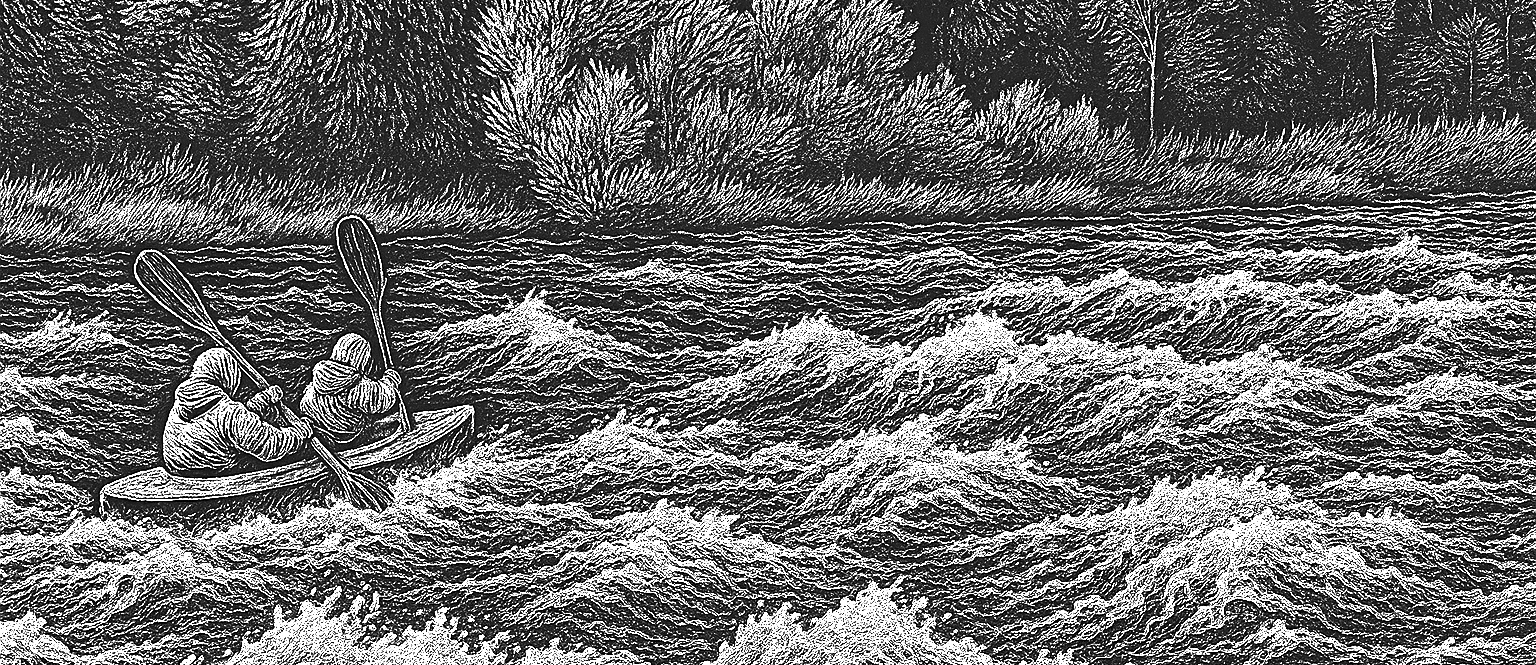
\includegraphics[width=1.0\textwidth]{36_3_zampolit}
	\caption{\small\textit{...Замполит как раз жёстко выгребал поворот...}}
\end{figure}
%\end{wrapfigure} 

Адмирал уже быстрее скакал по~шатающимся валунам обратно к~байдарке, ему не терпелось устроить Замполиту разнос. А~тот как чувствовал, что по~его душу мчится по~камням разозлённый Адмирал, и~просквозил дальше по~реке, не став останавливаться.

\diagdash Не, ну вы видали?!\mdash орал Адмирал.\mdash Ваще ни~стыда, ни~совести!!! Ну, ёклмн!!!

\diagdash Да забей, щас мы их нагоним, садитесь давайте уже.\mdash Паша стащил байду с валунов, смотал чалку, начал усаживаться. 

Адмирал с Русланом последовали его примеру, быстро залезли в байду и, закрыв юбки, начали выгребать к~середине русла. Замполит, тем временем, уже давно скрылся за~следующим поворотом. Догнать второй экипаж Адмирал никак не поспевал\mdash те нырнули в следующий порог\mdash Ковеланлиете\sdash Коски, который представлял собой сплошную бурлящую шиверу длиной метров 700.

Читать лоцию адмиральский экипаж, конечно, не~мог, поскольку та была в замполитовском телефоне, поэтому они ломились вперёд так, полагаясь на~удачу. Адмирал успел во~время остановки на каменной гряде посмотреть в навигатор и~вспомнить, что Ковеланлиете\sdash Коски будет достаточно протяжённым:

\diagdash Парни, аккуратно, гребём ровно, не упираясь. Порог будет длинным, но вроде без жести!

\diagdash Сань, ты рули давай!\mdash Паша сел поудобнее насколько мог.

\diagdash Ага! Готовы? Юбки закрыли?

\diagdash Готовы!!!

Они вал за валом прошли первую половину порога по~самой середине русла, и им предстала картина белой водяной каши, уходящий за правый поворот, где мгновения назад скрылся замполитовский экипаж.

\diagdash У, черти! За ними!!! {\large ПОЛНЫЙ НАХОД!!!}\mdash подгонял Адмирал свой экипаж, а сам тихонечко выруливал правее под берег, обходя метровые валы по центру. 

Они легко прошли очередной порог, завернув направо, следуя изгибу русла. Только пройдя поворот, они увидели второй экипаж, вставший против течения у левого берега и ожидающий их. Адмирал повторил их заход от центра русла к берегу и тоже встал против течения. Наконец, они сцепились бортами.

\diagdash Парни! Ну, вы, блин, даёте!!!\mdash Адмирал жаждал замполитовой крови.

\diagdash Шурик, спокуха, рация сдохла$\ldots$\mdash доложил Замполит.\mdash И мы сначала ждали, ждали, а потом гляжу\mdash рацейка\sdash то тю\sdash тю. Ну~и~пошли. Извиняй~уж.

Адмирал всё понял и~мгновенно остыл\mdash отказ рации всё объяснял.

\diagdash А чего с ней?\mdash только и спросил он.

\begin{wrapfigure}[12]{r}{0.48\textwidth}
	%\begin{figure}[h]
	\centering
	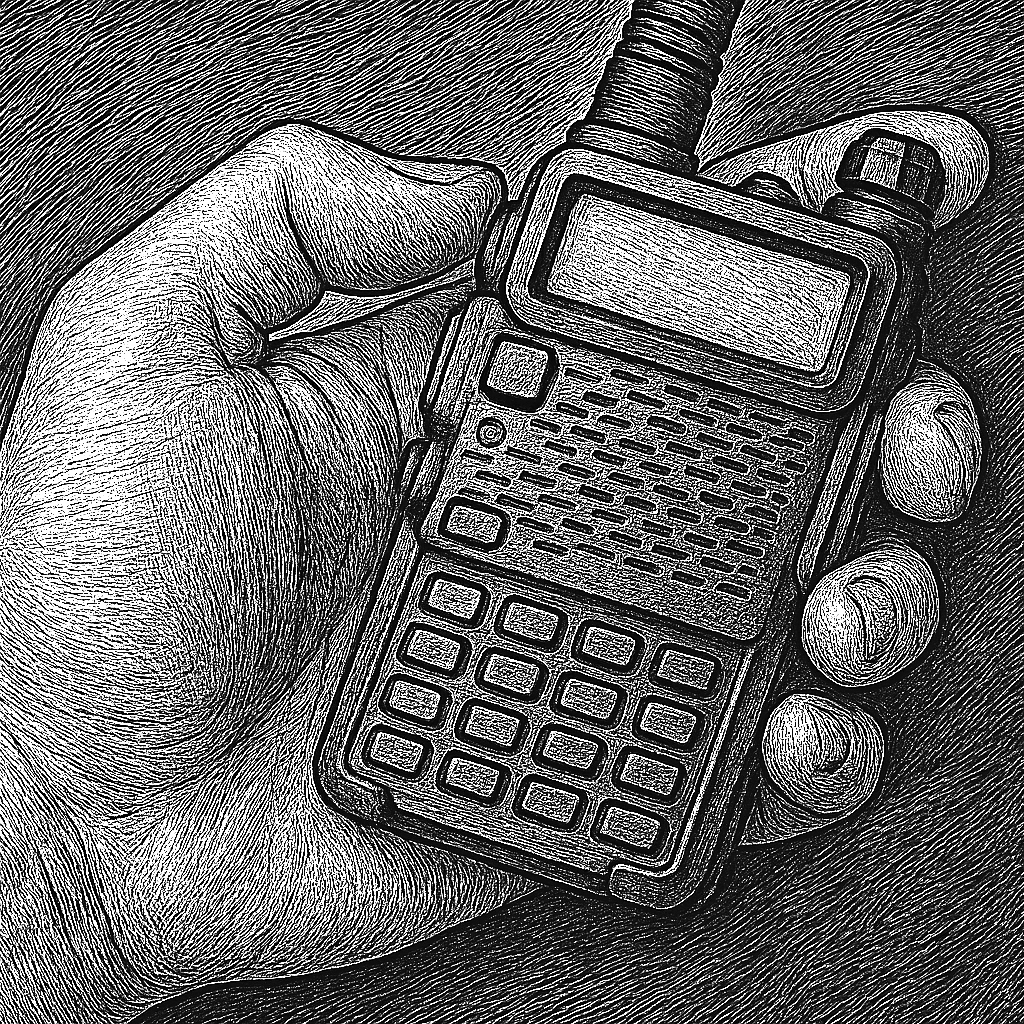
\includegraphics[width=0.46\textwidth]{37_1_radio}
	\caption{\small\textit{...спокуха, рация сдохла...}}
	%\end{figure}
\end{wrapfigure}

\diagdash Кнопку жмёшь и всё, экран гаснет, на.\mdash передал ему прибор Замполит.

\diagdash Ты её, засранец, позавчера не вырубил,\mdash догадался Адмирал.\mdash она у~тебя всю днёвку включённая была, сто процентов, вот аккумулятор и~сел в~ноль!!!

\diagdash Так ты не сказал$\ldots$

Адмирал уже набрал полные лёгкие разразиться матерной тирадой, но~удержался и только сказал, выдохнув:

\diagdash Перекурим?

\diagdash Давай$\ldots$\mdash согласился Замполит.

Они стояли, сцепившись бортами, под берегом и~приходили в себя от гр\'ебли: 

\diagdash Кстати, парни. А <<бочку>>\sdash то из описания кто\sdash нибудь заметил? Мы, например, нет. 

\diagdash И мы нет. Но там чё\sdash то такое слева было нехорошее, как мне показалось. Уж не знаю <<бочка>> это была или не~<<бочка>>.\mdash рассуждал Серёга.

\diagdash <<Бочку>> бы ты заметил,\mdash Замполит затушил папиросу,\mdash это была не она.

Серёга допил чай и спросил:

\diagdash А долго нам ещё сегодня?

<<Первый признак усталости>>,\mdash подумал Адмирал, а~вслух сказал:

\diagdash Щас глянем.\mdash и достал навигатор.

Руслан перезацепился за байду Замполита и достал свой термос~с~чаем:

\diagdash Да в принципе норм ещё, можем идти и идти!

\diagdash Серёг, ты погляди, какого м\'{о}троса ты откопал! Ему~хлеба не надо, весло подавай! Ы-ы-ы!

\diagdash Ы-ы-ы\mdash заржали все.

\diagdash Так!\mdash Адмирал промерил путь в навигаторе.\mdash Нам~примерно километров 8 осталось, но тут ещё 5 порогов.

\diagdash Хренас-с-cе!

\diagdash Как есть, а шо не так?\mdash Адмирал закрыл термос и~убрал его под фартук.

\diagdash Погнали тогда, какой следующий порог?\mdash Паша закрывал юбку.

\diagdash Леполису.

\diagdash Чё пишут?

\diagdash Кирь, прочтёшь?\mdash попросил Адмирал.

\diagdash Шивера пишут на 300 метров, проход справа, осмотр затруднён.

\diagdash И всё?

\diagdash Ну.

\diagdash Фигня после Уйтуженкоски, отчаливаем!\mdash Адмирал оттолкнулся рукой от замполитовой байды и правым находом вышел на стремнину.\mdash Не отставайте теперь уже, держимся вместе, не расходимся из прямой видимости, радиосвязи нет!

Адмирал разглядел главную струю порога и прошёл справа по самой её кромке, стараясь ровно\sdash ровно на ней держаться, в чём ему активно помогал экипаж. В середине порога им открылся шикарный вид на широченный разлив, и они, взяв ещё правее, не гребя, вышли на~простор.

\diagdash Уже как\sdash то неинтересно, что ли.\mdash сказал разочарованно Паша, обернувшись назад.

\diagdash Ну почему, тоже неплохо! Мы мастерски с вами по самому гребню прошли.\mdash сказал довольный Адмирал, заложив левый поворот.

\diagdash Да ваще по лайту!\mdash Руслан окончательно, надо полагать, освоился.

Далее на протяжении где\sdash то двух с половиной километров им встретилось три лёгких, ничего особенного собой не представляющих, порожка, которые они без осмотра и чтения лоции успешно прошли.

Эскадра размеренно гребла навстречу новым приключениям. Настрой у всех стал поуверенней.

\diagdash Тащ Замполит, лоция!\mdash повелевал Адмирал.

\diagdash Так тощн! Та-а-ак! Следующий\mdash порог Сухой.

\diagdash Эт я знаю, ты описание гони.\mdash Адмирал смотрел в~GPS\sdash прибор.

Они, не гребя, шли по инерции почти параллельно друг другу по~руслу, вода была спокойной, затишье перед Сухим.

\diagdash Что\sdash то не нравится мне его название\mdash <<Сухой>>.\mdash почти синхронно сказали Серёга с Русланом.

\diagdash Не очкуйте, м\'{о}тросы! Усё будет тип\sdash топ!\mdash хорохорился Адмирал и, обратясь к Замполиту, продолжил.\mdash Кирь, ну чё ты там?

\diagdash Ща! Шурик, очень неудобно рулить байдой и~одновременно читать, прикинь!\mdash он то и дело подруливал веслом.\mdash Так! Рекомендуют идти справа, муть какая\sdash то.

\diagdash Спокойно, не очкуем. Выстраиваемся в кильватер за~мной и потихоньку заходим. 

\diagdash Шурик, а ты видишь КУДА заходить?

\diagdash Давайте по центру, вроде в боковых протоках хуже, что слева, что справа!

\diagdash Ух, ё! Ну погнали!\mdash Замполит чуть подотстал и стал повторять адмиральскую траекторию.

\diagdash Нормально, нормально! Малый ход, парни!!!\mdash крикнул Адмирал и взял чуть правее, а дальше на~протяжении метров двухсот лавировал между камнями.\mdash Ёпрст! Реально сухой, ну!

А дальше взору сплавщиков открылся широченный разлив\mdash ещё шире, чем после Леполису\mdash и вторая ступень Сухого, представленная огромной <<стрелкой>> с ярко выраженным <<языком>>. Адмирал решил править по самой кромке <<языка>>, осторожно не суясь в центр.

Едва пройдя вторую ступень, ребята увидали выход из~порога с третьей ступенью и ярко выраженным сливным бурлением по центру и белеющим <<языком>>:

\diagdash Да ну нахрен!!!\mdash выругался Адмирал и взял к~левому берегу.\mdash Там глубже, я не хочу напрямки ломиться!!!

%\begin{wrapfigure}[12]{r}{0.48\textwidth}
	\begin{figure}[h]
	\centering
	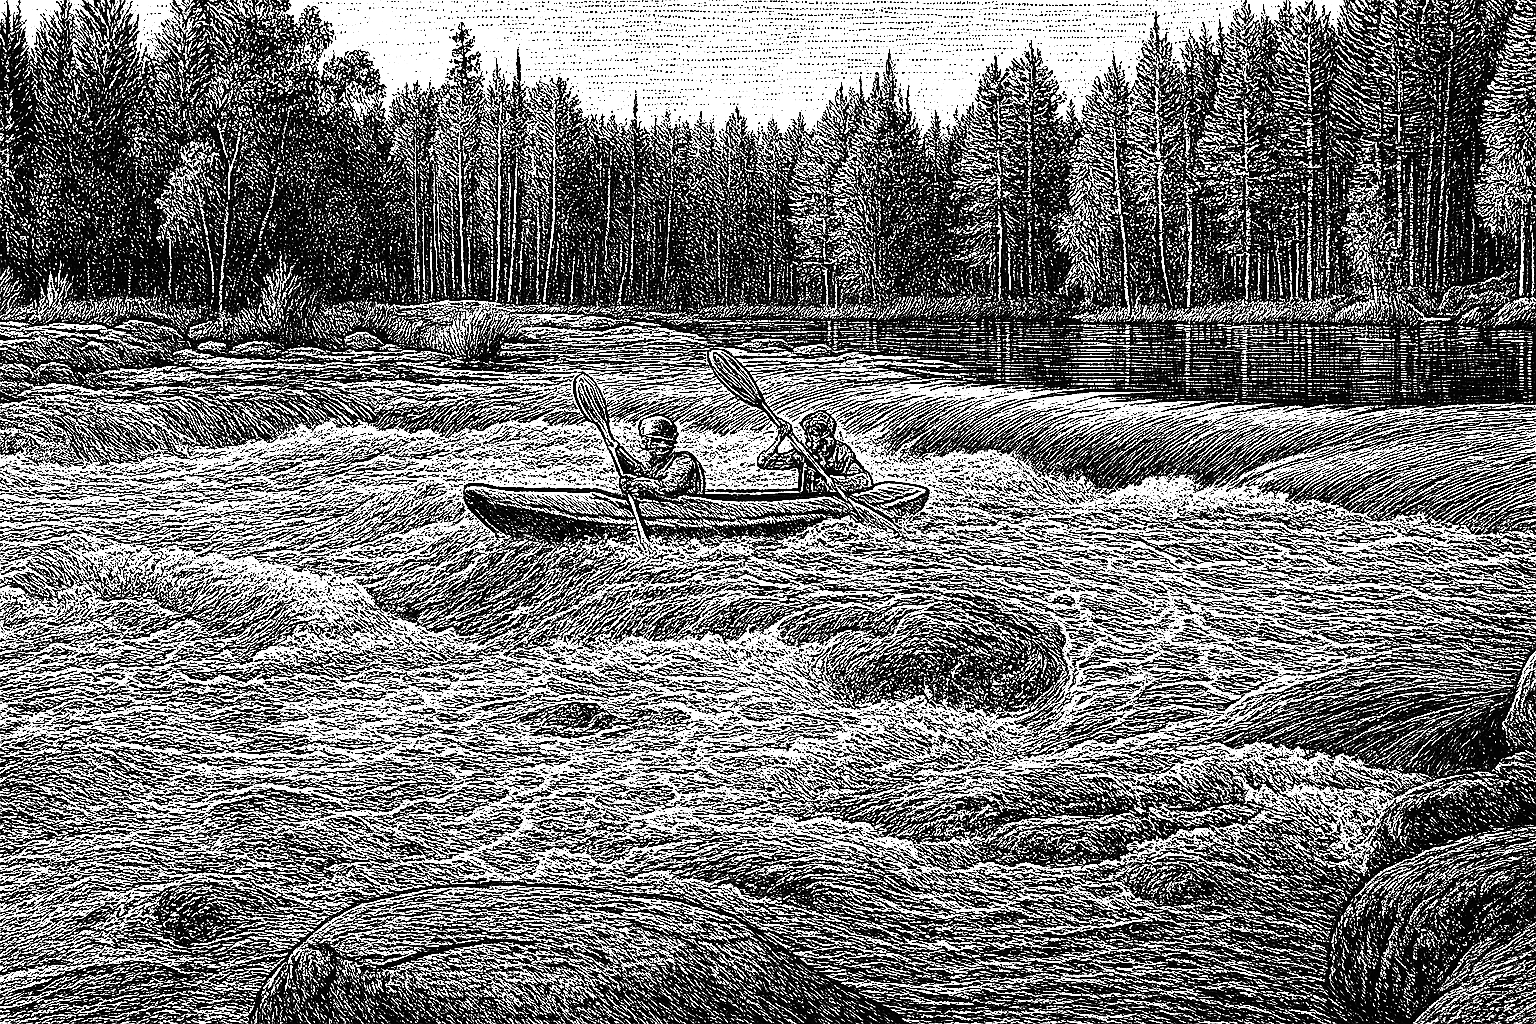
\includegraphics[width=1.0\textwidth]{38_1_suhoi}
	\caption{\small\textit{...ребята увидали выход из~порога...}}
	\end{figure}
%\end{wrapfigure}

\diagdash Уходим левее!!!\mdash успел проорать Замполит, и они нырнули в левую протоку, огибая самую жесть по центру.

Из\sdash под левого берега они сделали выход к центру после широкого слива и вышли на середину русла, увлекаемые пенящимся потоком дальше.

\diagdash ПРОШЛИ!!!\mdash орали они на всю округу.

\diagdash Да, но как\sdash то без огонька, что ли?\mdash раздосадованно добавил Паша.

\diagdash Просто воды больше, мы же всё ниже и ниже по~течению идём. Пороги всё менее жёсткими становятся.\mdash пояснил Адмирал и стал потихонечку править к центру разлива.\mdash Надо бы дальше описание. Кажется где\sdash то после Сухого обещали стоянку.

\diagdash Да???\mdash народ оживился.\mdash Гребём, давайте!!!\mdash всем уже хотелось причалить и развернуть лагерь.

\diagdash Не торопитесь, времени ещё хватает. Ищем стоянку спокойно.\mdash Адмирал размеренно грёб, довольный прохождением Сухого.

Посреди разлива Адмирал углядел лишь одно место под стоянку на правом берегу, но вид с воды никому не~понравился, они пошли дальше.

\diagdash Шурик, уже бы на стояночку, скоро солнце начнёт заходить, а нам бы просушиться ой как не мешает.\mdash справедливо заметил Замполит.

\diagdash Ну а что я тебе сделаю? Гребём, ищем!\mdash тот копался в навигаторе и подправлял курс, пока его экипаж загребал.

\diagdash Чё там, тащ Адмирал?

\diagdash Чё, чё. Порог Каданлоама, готовимся морально.

\diagdash Скоро? 

\diagdash Буквально километр!

Километр просквозил незаметно, и маленькая эскадра устремилась в бурлящую гущу очередного порога, про~который было сказано, что это простая шивера длиной около трёхсот метров без каких\sdash либо сложностей.

\diagdash По главной струе, парни! Айда за мной! И-ха!\mdash надрывал Адмирал связки, жёстко загребая к центру.

\diagdash Са-а-аня! Ты уверен?\mdash Паша под конец устал маленько.

\diagdash Стопроц! Погнали, мужики!

Они легко прошли по главной струе достаточно мощный, но беспроблемный порог. Второй экипаж последовал за ними, даже обогнав на выходе, поскольку Адмирал отвлёкся на навигатор.

\diagdash Тэк-с. Ну и?\mdash Серёге было интересно где они найдут стоянку среди берегов, опять ставших низкими после Сухого.

\diagdash Спокойствие, только спокойствие. В разливе после Каданлоамы должна быть стоянка. Здесь Черанга впадает справа, вот тут и ищем!

Они прошли весь разлив, но так ничего и не нашли, как~ни~всматривались в берега.

\diagdash Ну? Где?\mdash команда требовала стоянку.

\diagdash Ну я рож\'{у} вам её, в самом деле? Ищем, ёпрст! 

Увлекаемая неслабым течением, эскадра стала заворачивать за правый поворот, где послышался шум порога Длинный.

\diagdash ПАРНИ, ПОПАДОС!!! РАЗВОРОТ!!! Копаем жёстко вёслами!!! Утянет в порог\mdash хрен выгребем!!! Стоянка в~том разливе позади нас, стопроц!!!

\diagdash Шурик, едрить твою!!!\mdash только и успели ответить экипажи. 

Все принялись выполнять разворот, борясь с~утягивающим течением. Этот манёвр дался им нелегко, они еле\sdash еле выгребли обратно в разлив и вышли на самую широкую его часть.

\diagdash Ну и где, тащ Адмирал, так и раз эдак, твоя неземных красот стоянка???\mdash Замполиту уже не терпелось.

\diagdash Ищем, Кирь. Я тут в первый раз, как и все.

\diagdash Куда идти-то?

\diagdash Да откуда я знаю? Пока просто против течения возвращаемся, щас может поймём.\mdash Адмирал мысленно вспоминал описания маршрута и вдруг его как осенило:\mdash Ну~вон~же! Вон выход к воде!\mdash аккурат среди буйной растительности зиял прог\'{а}л. Он моментально понял, почему они сразу не заметили эту стоянку\mdash для этого надо было почти сразу после прохода Каданлоамы обернуться и~посмотреть назад. Он заорал:

\diagdash Эврика! Прямо по курсу стоянка!

\diagdash Ты угораешь? Где?!\mdash экипажи в упор не видели очевидного.

\diagdash Да вон! Прямо по курсу! Внимательнее, вон подъёмчик среди зелени!

Они стремительно неслись к небольшой полосочке песочка, около которой находился большой валун и далее вверх вглубь леса уходила тропка.

\diagdash А точно! Глядите\sdash ка!\mdash Серёга обрадовался.

\diagdash А ты думал, я гоню что ли?

\diagdash Да ни в жись!

\diagdash То-то же, смотрите у меня! Всем приготовиться! Заходим правым бортом к берегу!\mdash Адмирал, потихоньку табаня, плавно заходил к подъёму своим любимым приёмом зачаливания.

<<Стоянка, скорее всего, в глубине. Хоть бы тут никого не было!>>\mdash мысленно подумал он. Они молниеносно высадились и, шлёпая по воде, вышли на берег:

\diagdash Ну, за мной, глянем$\ldots$\mdash Адмирал зашагал вверх по~подъёмчику.

Взору разведчиков открылась небольшая поляна, баня, костровище шикарное с огромными скамейками\sdash брёвнами и~полное отсутствие мест под палатки. Лес вокруг был мокрый\sdash премокрый после утреннего дождя, не успел просохнуть за целый день.

Адмирал походил, побродил с веслом по стоянке, забил себе и Замполиту место под палатку под огромной елью:

\diagdash Остаёмся, ясен красен!

\diagdash Пф! Ещё б! Место каеф!

\diagdash Ну!

\diagdash Так, оп-оп-оп, мужики! Мутим всё в темпе, жрать хочется просто жесть после ходового дня! Айда, на разгрузку!

\diagdash Шу-у-урик, это остров!\mdash сказал вернувшийся из~разведки Серёга.\mdash там дальше в лесочке протока.

\diagdash Крутяк! Робинзоним опять! Погнали снарягу перетащим сначала, потом всё остальное.\mdash Адмирал семимильными шагами топал к берегу.

Они в темпе перекидали вещмешки на берег, затащили и перевернули байды, всё как обычно. Затем перенесли гермы с продуктами поближе к костровищу. Адмирал оценил, что прикостровых дров хватит им на сутки и более\mdash кто\sdash то до~них напилил тут впрок бензопилой огромные брёвна.

\diagdash Так, внимание всем! Эскадра, слушай мою команду! Всем переодеваться в сухое!\mdash скомандовал Адмирал и~принялся потрошить свою герму, чтобы достать сухие штаны и тельняшку.

Все были только рады, а Паша, надо полагать, более всех. Переодевшись, сплавщики собрались у~костровища. Адмирала захватила эйфория от сплавного дня:

\diagdash Парни, надо за сегодняшний день, живо! Больше половины порогов~прошли! Первые~настоящие~пороги!!!% в наших сплавах!!! 

\diagdash Ну!!!

\diagdash Паш, подсоби?

\diagdash Не представляешь, с удовольствием, почти что первый раз за день!\mdash тот достал закуску и разложил её на бревне, сделав импровизированный столик.

Адмирал достал из гермы очередную тару:

\diagdash На сегодня у нас Гран Аньехо, волки вы речные, так и раз эдак!

\diagdash Шурик, тут грибов куча вокруг полянки и ягод, мы пойдём наберём с Русланом.\mdash известил вернувшийся из~разведки Серёга.

\diagdash Погодь, надо эц-самое!

\diagdash Ну давайте!

\diagdash Замполит, там узбекский лимон был, порежь его?

\diagdash Тащ Адмирал, как понять, что он узбекский???

\diagdash Сердцем!

\diagdash Ы-ы-ы!

\diagdash Ладно-ладно! Он оранжевее остальных.

Когда всё было готово, Замполит включил запись видео в телефоне. Адмирал взял две дольки лимона и осведомился:

\begin{wrapfigure}[17]{r}{0.5\textwidth}
	%\begin{figure}[h]
	\centering
	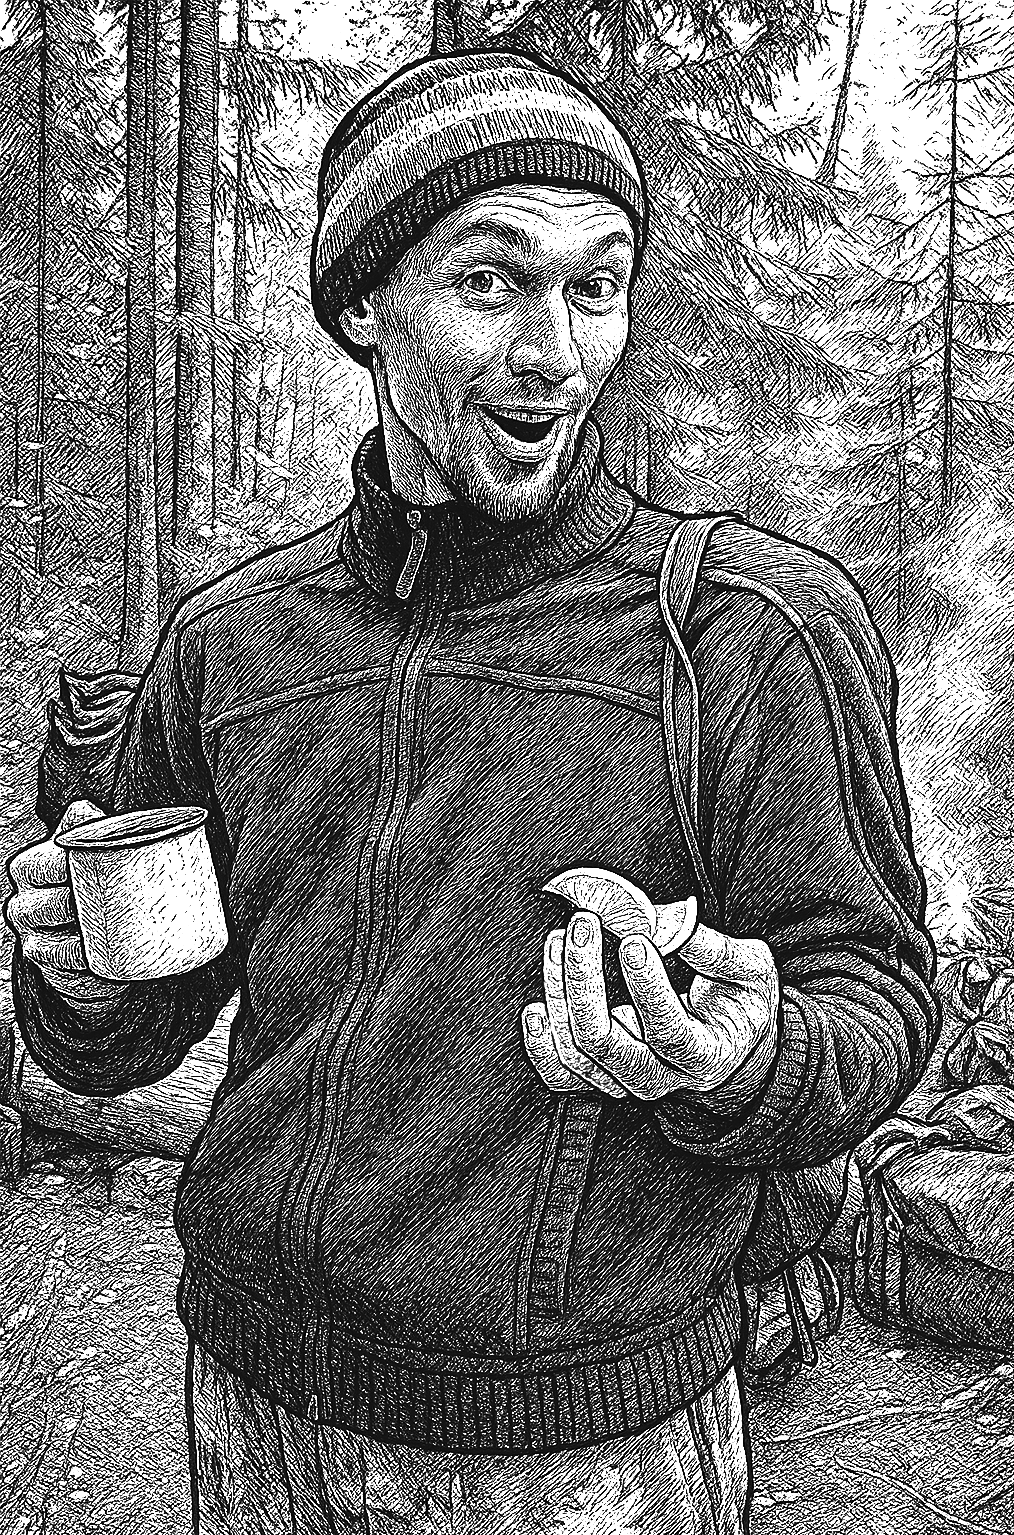
\includegraphics[width=0.46\textwidth]{39_2_rum}
	\caption{\small\textit{...чай, лимон, всё харашо!..}}
	%\end{figure}
\end{wrapfigure}
\diagdash Можно уже, да?

\diagdash А то!

\diagdash Итак, мужики!\mdash начал Адмирал, пародируя акцент.\mdash Там шумит порог Каданлоама! Мы стоим тут на~островэ! У нас есть$\ldots$\mdash он посмотрел в кружку, полную кубинского рома,\mdash $\ldots$чай, лимон, всё харашо! Да? Мы~переоделись в сухоэ, одэжда у нас вон там на вэрёвочке сушится висит! Кирь, засними эту выставку\sdash продажу! Вон~там всё сушится$\exldots$%!$\ldots$


\diagdash После героического прохождения порогов!\mdash вставил Паша.

\diagdash Естественно!!!\mdash продолжил Адмирал.\mdash Всего\sdash то вторая категория, а как будто пятую прошли! И прошли на <<отлично>>! Ну, режиссёр, заканчивай съёмку. За~прохождение! Два~отрывистых и одно раскатистое!

\diagdash {\large УРА, УРА, УРА\sdash А\sdash А!!!}\mdash грянуло над островом.

\diagdash Ай, хорошо!\mdash парни с наслаждением закусили потрясающим лимоном.

\diagdash Спрашиваешь! Сладкий лимон\mdash тема!

\diagdash Пф, обижаешь! Профи в теме.

\diagdash А как мы сегодня прошли, а? Вначале\sdash то как все ссали? А? Ну? Что, не так что ли было?

\diagdash Ну было, было. Уймись, Шурик.

\diagdash Потом зато как разошлись, орлы!

\diagdash Шурик, между первой и второй!

\diagdash Аз есмь!

\diagdash Ну, давайте, по второй и костёр делать!

\diagdash Широка\sdash а\sdash а страна\sdash а\sdash а моя\sdash я\sdash я роодна\sdash а\sdash ая, многа\sdash а\sdash а в не\sdash е\sdash ей лесо\sdash о\sdash ов, поле\sdash е\sdash ей и ре\sdash е\sdash ек! Я~друго\sdash о\sdash ой такой страны не зна\sdash а\sdash аю, где так счастлив мог быть челове\sdash е\sdash ек!\mdash пропел Адмирал и пошёл колоть дрова$\ldots$

\vspace{0.5cm} 
$\ldots$Серёга притащил из лесу полкотелка черники:

\diagdash Гляньте! Кр-р-расота?

\diagdash Ваще-е-е! Где нарыл?\mdash Киря сфоткал урожай.

\diagdash Да прям вон не сходя с острова!

\diagdash Замполит, ставь воду на компотик! Ы\sdash ы\sdash ы!\mdash Адмирал суетился с ужином у пылающего костра.

\diagdash Однозначно!\mdash ответил тот и направился к реке набрать воды.

На берегу, тем временем, Паша уже разложил своё рыбацкое хозяйство и пробовал половить\mdash вдруг вытащит чего к ужину. 

\diagdash { \large ВОТ ОНА, ВОТ ОНА, ОП\sdash ПАЧКИ!!!}\mdash донеслись до~костра вопли Замполита от берега.

\diagdash Чё у них там?\mdash Адмирал вскрывал банки с~тушёнкой на суп.

%\begin{wrapfigure}[15]{l}{0.6\textwidth}
\begin{figure}[h]
	\centering
	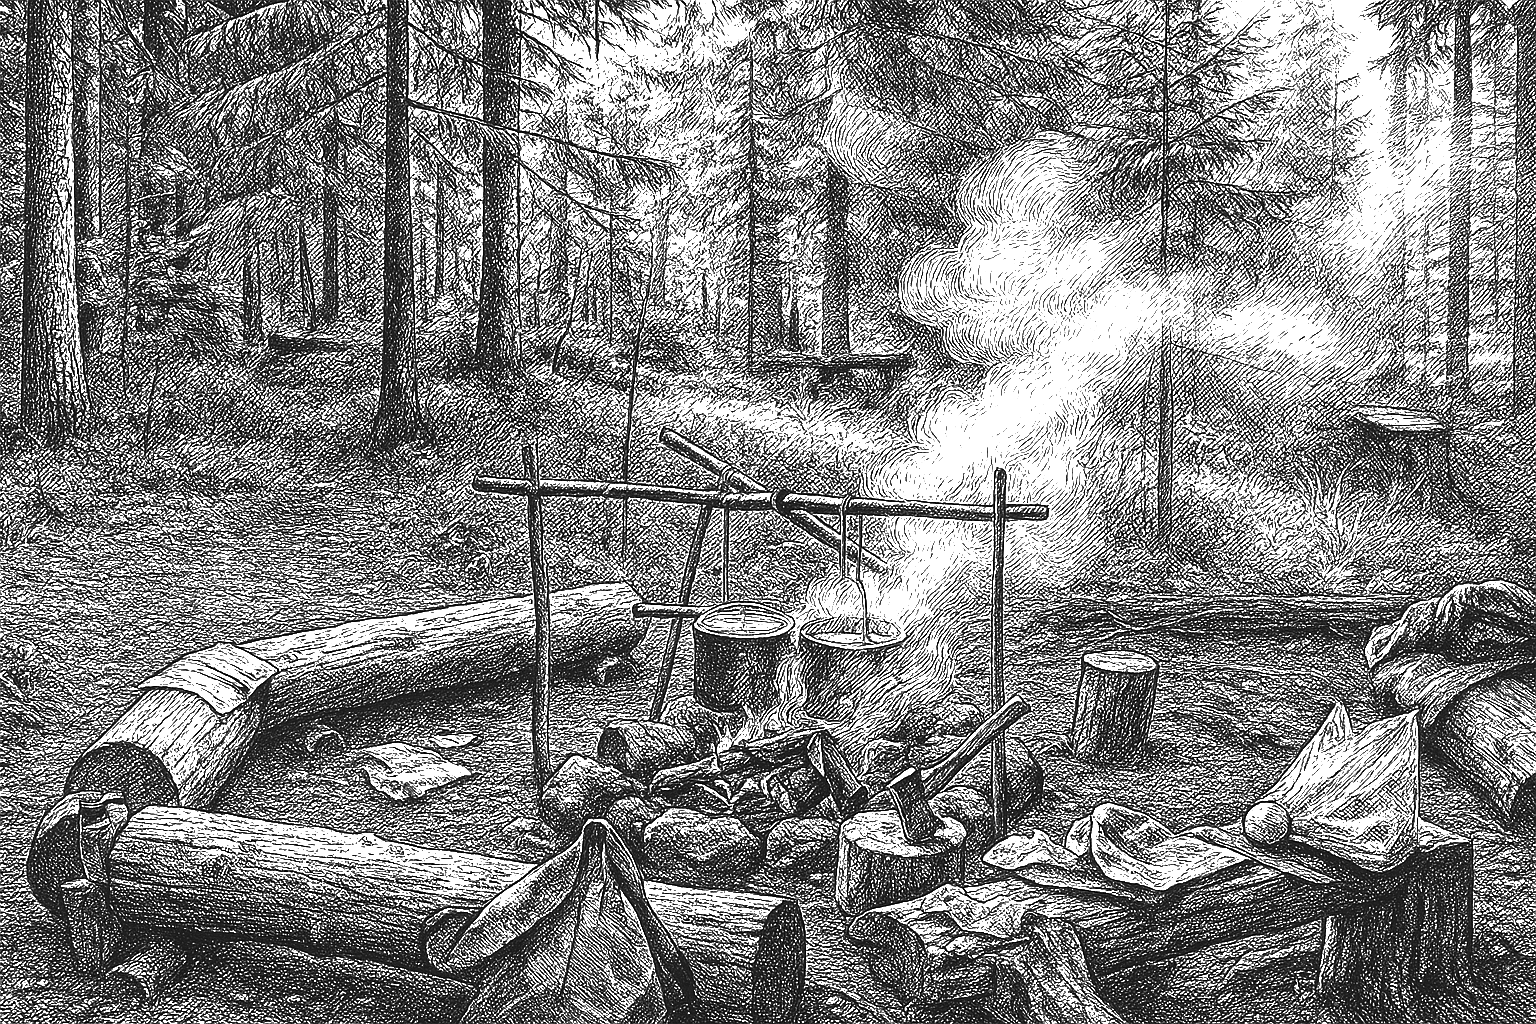
\includegraphics[width=1.0\textwidth]{40_1_fire}
	\caption{\small\textit{...у пылающего костра...}}
\end{figure}
%\end{wrapfigure}

Замполит вернулся от берега с полным котелком воды и горящими глазами:

\diagdash Пашка щуку вытащил! Во такенную!\mdash он хотел показать руками, но те были заняты котелком. Замполит повесил котелок над костром и принялся показывать размеры гигантской щуки, все заржали.

Адмирал почти закончил с ужином и пошёл на берег помыть руки:

\diagdash Ну как тут у тебя, тащ Рыбак?\mdash окликнул он Пашу.

\diagdash Гляди какая! Ух!\mdash тот поднял щуку и показал Адмиралу.

\diagdash Класс!!! Поздравляю! Зажарим?

\diagdash Зажарим!

В этот момент на разлив после Каданлоамы высыпалась огроменная флотилия, та самая, без сомнений, которую они обогнали на Нурмисе:

\diagdash Глянь, Сань.\mdash Пашка показал на них.

\diagdash Ага. Ну, что я могу сказать, они тормознуто идут, у~них же катамараны.

Цветастая флотилия шла дальше вниз по~течению, вереница лодок, каяков и катамаранов растянулась в~длиннющую цепочку. Адмирал отмыл руки и собирался обратно к костру:

\diagdash Давай приходи, там почти всё готово.

\diagdash Ага!

Пацаны, тем временем, собрались у костра в кружок:

\diagdash А зачем печь вон та каменная?\mdash спросил Руслан, указывая на груду камней у самого спуска к берегу.

\diagdash Это? Ты чо-о-о! Это божественная штука! Это\mdash банная печь! Её надо топить где\sdash то полдня, чтобы камни прям капец как раскалились, а потом накрыть сверху тентом и усё\mdash готово, можно париться! Вещь улётная, но у нас тента нет соответствующего,\mdash Адмирал попробовал суп и~продолжил,\mdash чтобы это всё провернуть. Мы вон когда с~женой ходили по башкирским рекам\mdash там это в порядке вещей, чуть не на каждой стоянке хорошей каменка есть.

%\begin{wrapfigure}[10]{l}{0.5\textwidth}
%	%\begin{figure}[h]
%	\centering
%	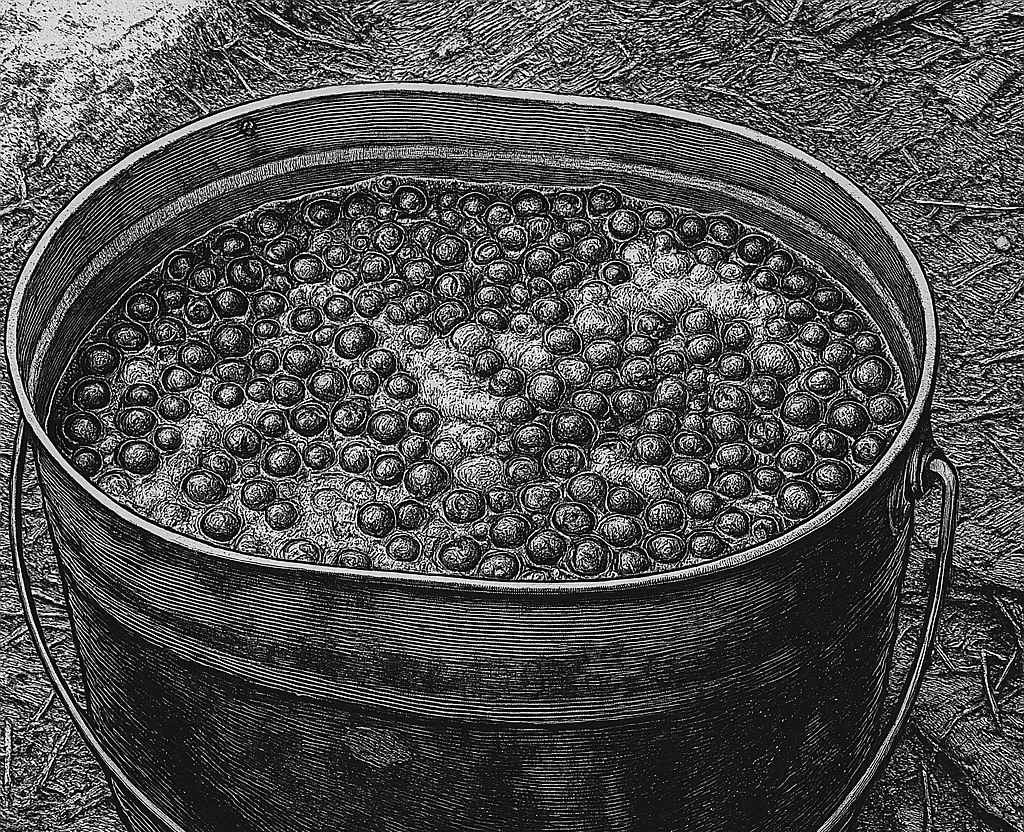
\includegraphics[width=0.46\textwidth]{kompotik}
%	\caption{\small\textit{...компотик...}}
%	%\end{figure}
%\end{wrapfigure}
%
\diagdash А почему тогда мы не~брали банный тент?

\diagdash Ну-у-у, его делать надо из чего\sdash то. И~потом\mdash возьмёшь, бывало, плёнку в~качестве тента с собой, а~камней нет печь сложить\mdash мы так по Лиди, помню, ходили. \makebox[\linewidth][s]{\noindent Ух,~чертыхались! Год ещё холодный был\mdash мокро, сыро,}

%\begin{wrapfigure}[15]{l}{0.6\textwidth}
\begin{figure}[h]
	\centering
	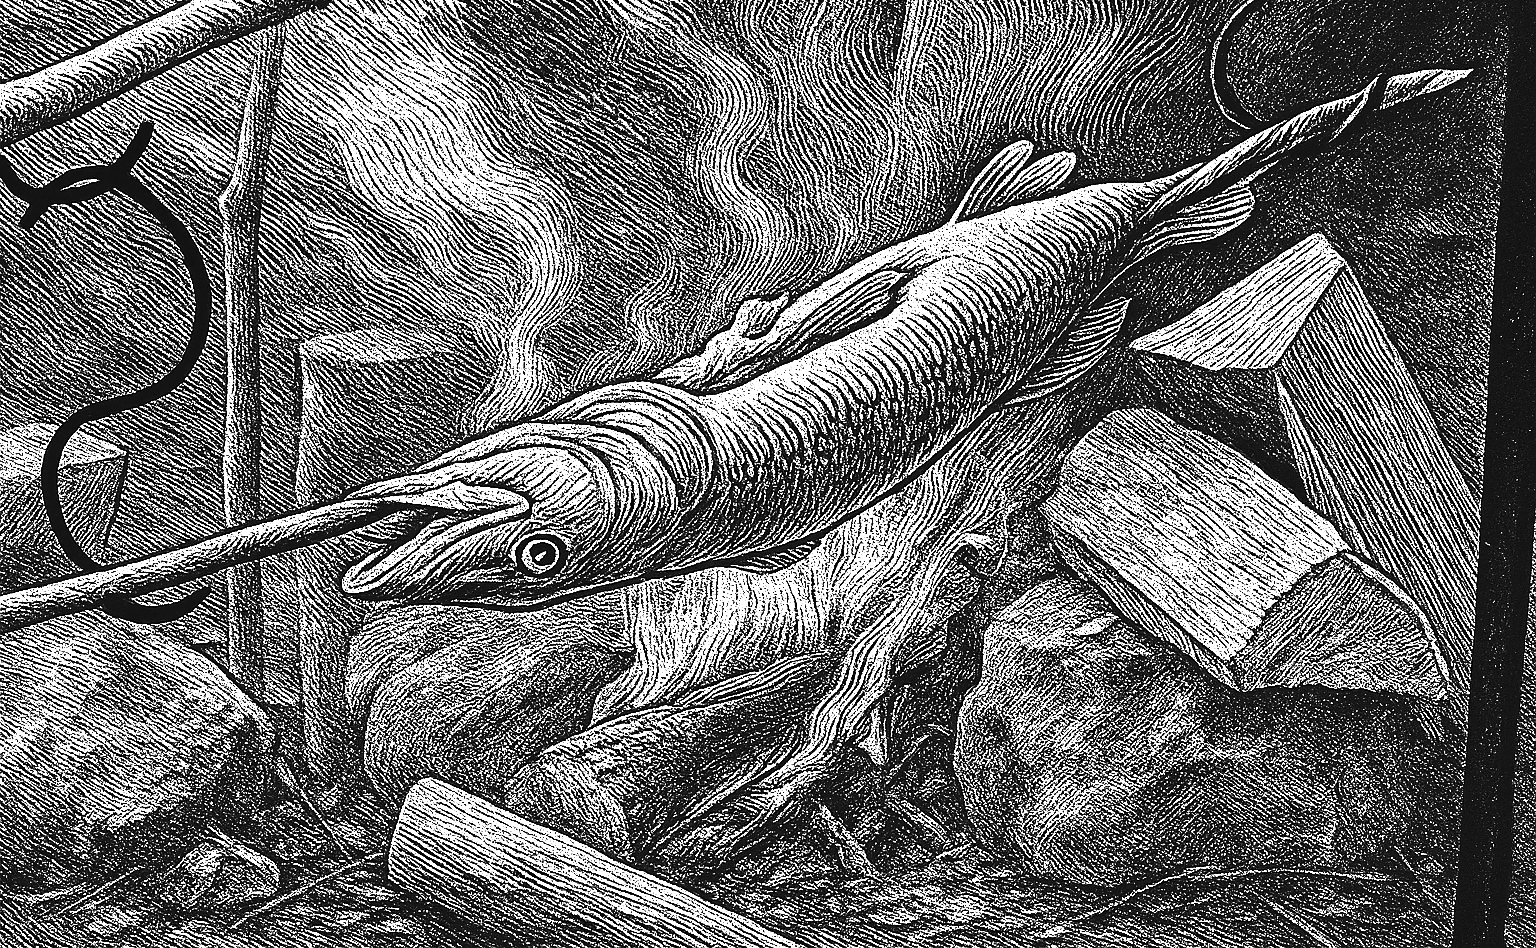
\includegraphics[width=1.0\textwidth]{41_1_pikefish}
	\caption{\small\textit{...ещё и щука под вечер...}}
\end{figure}
%\end{wrapfigure} 

\noindent банька бы в тему пошла, а камней нет. Так и провозили весь поход эту плёнку без толку, эх,\mdash вспомнил Адмирал былое.

\diagdash А из нашего дождевого тента сделать если?

\diagdash Маловат он по площади. Я уже думал над этим. Баня, как новое слово в~наших путешествиях, у нас ещё впереди, парни!

\diagdash Шурик, я б не~отказался.\mdash заявил Замполит.

\diagdash Да кто б отказался-то!\mdash Адмирал попробовал суп и~традиционно зазвенел крышками котелков, созывая народ к костру:\mdash Айда ку\sdash у\sdash ушать!

Паша пришёл с берега с потрошённой щукой и, насадив её на берёзовый прутик, повесил горизонтально над костром на крюках:

\diagdash Во! А то тушёнка всё, да тушёнка! Класс?

\diagdash Спрашиваешь! Конечно класс.\mdash Адмирал раскладывал порции ужина.\mdash Сегодня ваще день улётный\mdash и дождь, и~солнце, и пороги, и стоянка классная, ещё и щука под вечер! А вечер\sdash то какой спускается, мужики! Звёзды будут!

\diagdash Да-а-а$\ldots$ Красота\sdash то какая!

Они, утолив голод, неспешно трапезничали, болтали и~ожидали пока подоспеет рыба$\ldots$

\vspace{0.5cm}
$\ldots$Прошло наверно не менее получаса, когда, перекусив, парни принялись фотографировать щуку, которая готовилась над костром:

\diagdash Когда запечётся?

%%\begin{wrapfigure}[15]{l}{0.6\textwidth}
%\begin{figure}[h]
%	\centering
%	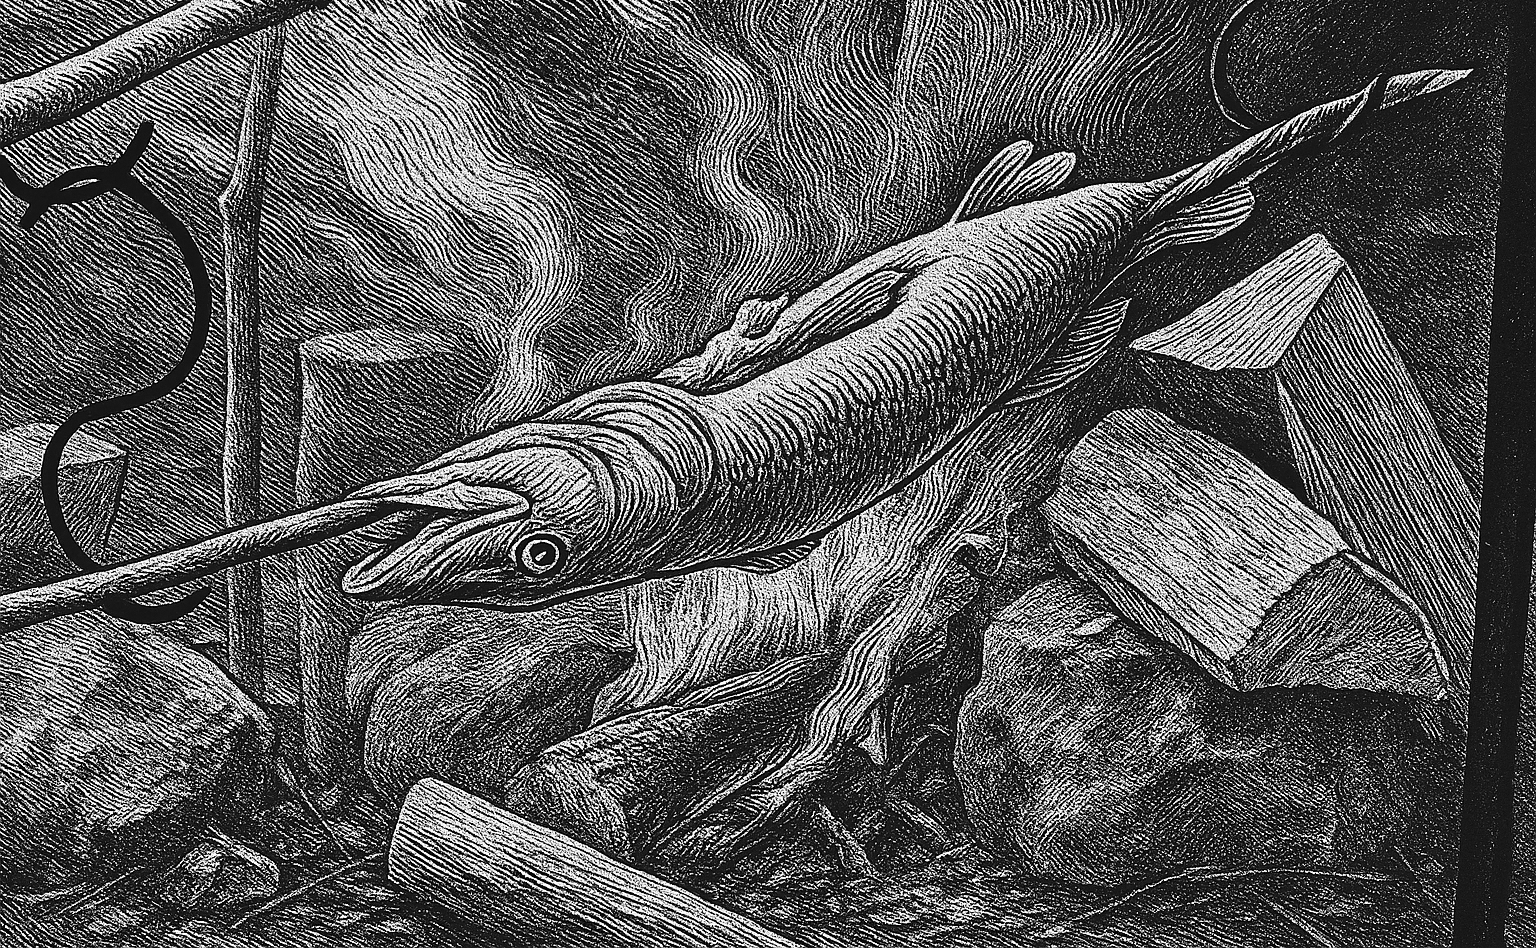
\includegraphics[width=1.0\textwidth]{fish}
%	\caption{\small\textit{...ещё и щука под вечер...}}
%\end{figure}
%%\end{wrapfigure}

\diagdash Ща погляжу.\mdash Пашка приоткрыл жабры палочкой.\mdash Почти готова!

\diagdash Класс! Такую огроменную рыбину ты первый раз по\sdash моему вытащил в наших походах?\mdash спросил Адмирал.

\diagdash Да наверно$\ldots$ Хотя на Лиди тогда лещару вытащили тоже не мелкого! 

\diagdash Было дело$\ldots$\mdash Адмирал откинулся в походном кресле.\mdash <<Бойцы вспоминают минувшие дни и битвы, где вместе рубились они>>.

Выждали ещё пару минут, Паша снял с костра щуку. Они разделали её и стали вкушать вкуснейшее белое филе:

\diagdash М-м-м!

\diagdash М-м-м-м!

\diagdash Харош, парни! Как будто голодали до этого. %\mdash чуть обиделся Адмирал.

%\diagdash М-м-м-м-м!

%\begin{wrapfigure}[15]{l}{0.6\textwidth}
%\setlength{\belowcaptionskip}{-10.0mm}
\begin{figure}[h]
	\centering
	
\includegraphics[width=1.0\textwidth]{42_3_cigar}
	\caption{\small\textit{...вечер проходил у них с ленцой...}}
\end{figure}
%\end{wrapfigure}

%\diagdash Харош, парни! Как будто голодали до этого.\mdash чуть обиделся Адмирал.

\diagdash Да ты попробуй!

\diagdash Таки уже! Офигенно! Просто офигенно!\mdash щука исчезла в мгновенье ока, будто и не было её\mdash настолько вкусной она оказалась.

%%\begin{wrapfigure}[15]{l}{0.6\textwidth}
%\begin{figure}[h]
%	\centering
%	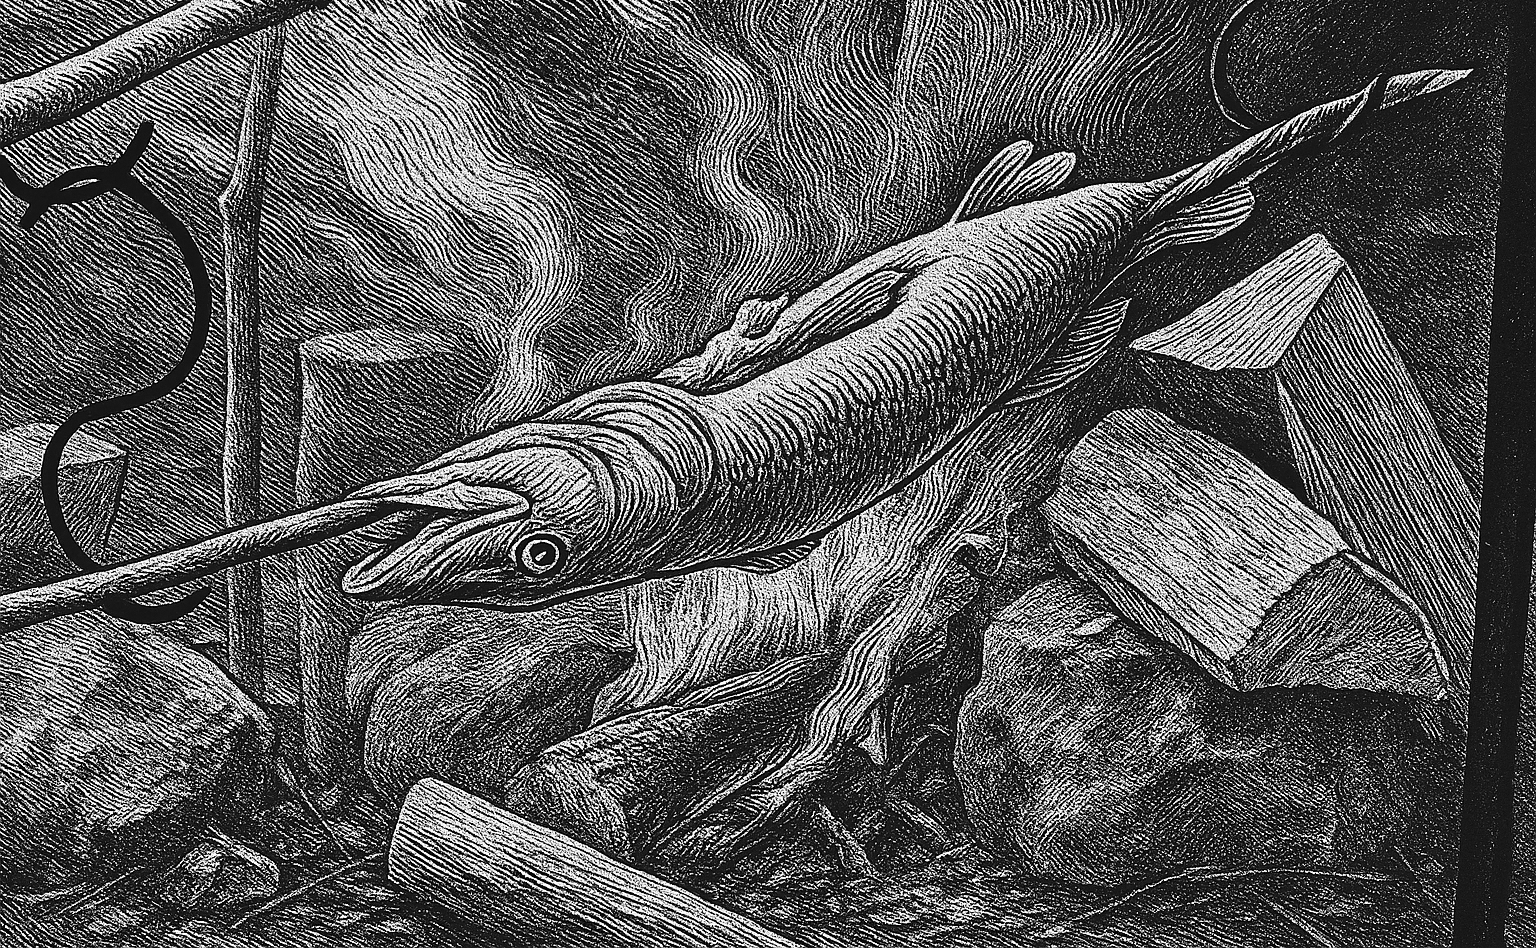
\includegraphics[width=1.0\textwidth]{fish}
%	\caption{\small\textit{...ещё и щука под вечер...}}
%\end{figure}
%%\end{wrapfigure}

Вечер проходил у них с ленцой\mdash сказывалась усталость за день. Они сидели вокруг костра, кто развалившись в~походных креслах, кто на брёвнах. Адмирал подсушил пенку, которая днём служила сиденьем в байдарке и которую он стелил в палатку ночью, и, уютно усевшись на неё в~кресло, достал сигару:

%Компотик сварился, каждый зачерпнул себе полную кружку. 

\diagdash Красота, мужики! Звёзды всходят первые, ночь красивая, только гляньте какой закат.\mdash через ветви высоченных сосен и елей, окружавших их стоянку, пробивались оранжево\sdash жёлто\sdash розовые краски.

\diagdash Ага, то есть восток, получается, у нас за спиной, за~этим дремучим лесом.\mdash Серёга показал на лес, что был позади них.\mdash Значит завтра солнышко не разбудит. 

\diagdash Да может облачно будет. Погодка\sdash то карельская переменчивая$\ldots$\mdash Замполит выпустил колечки дыма.

\diagdash Ну солнце в тучку садилось.\mdash Адмирал поправил свою раста\sdash шапку и~раскурил сигару. 

\diagdash Шу-у-урик, день был улёт.\mdash протянул Серёга.

\diagdash Да уж! Завтра вторая половина порогов.

\diagdash Сколько там?\mdash поинтересовался Паша.

\diagdash Порогов? Сколько ни есть, все наши! Ы\sdash ы\sdash ы\mdash заржал Адмирал.

\diagdash Ну глянь, интересно.\mdash попросил Серёга.

Адмирал достал свой командирский планшет и~сориентировался, взяв нужный лист карты:

\diagdash Так, ну вот. 4 порога ещё.

\diagdash Четы-ы-ыре? Всего\sdash то! А чё так мало? Получается, почти все сегодня прошли.

\diagdash Согласно плану, Серёг. Там потом Суна совсем широченной станет, слева Сямча впадёт. В устье на мысу хочу попробовать на стояночку встать.

\diagdash Да чё щас загадывать, посмотрим.\mdash Замполит потягивал чаёк.

\diagdash Карта мелкая, горизонтали редкие, фиг поймёшь чё~там за местность.

\diagdash Да какая разница? Придём, увидим, заценим$\ldots$

%\vspace{1.0cm}

\setlength{\belowcaptionskip}{1.0mm}

%\begin{wrapfigure}[15]{l}{0.6\textwidth}
\begin{figure}[h]
	\centering
	%	\includegraphics[width=1.0\textwidth]{11_5}
	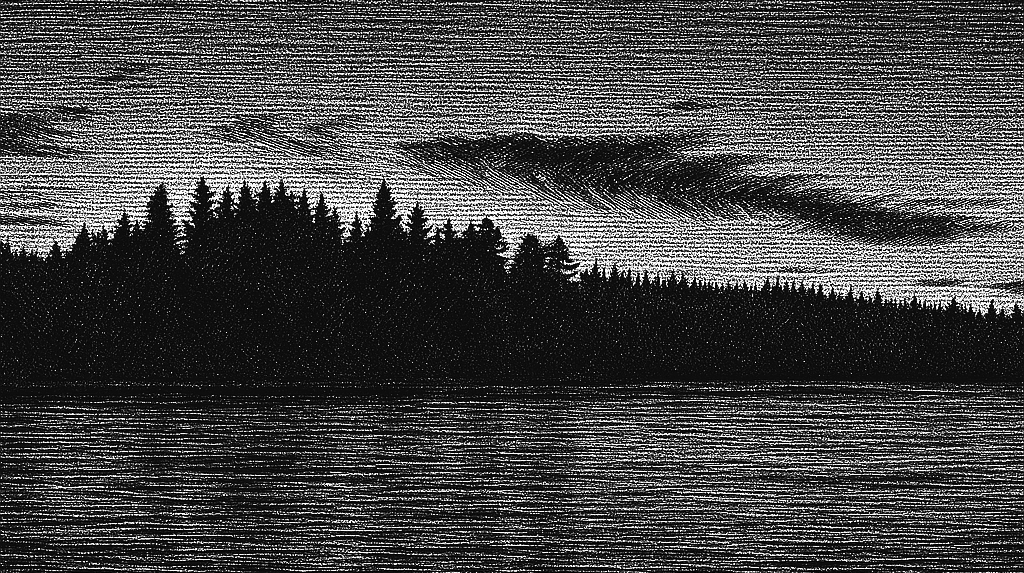
\includegraphics[width=1.0\textwidth]{43_1_cheranga}
	\caption{\small\textit{...Адмирал сходил к берегу пофотографировать разлив Черанги...}}
\end{figure}
%\end{wrapfigure}


%\newpage
$\ldots$Парни засиделись у костра далеко за~полночь, несмотря на~усталость. Свежесваренный компотик из~собранной Серёгой черники вышел наварист и уходил просто на ура, они выпили почти весь котелок. Адмирал сходил к~берегу пофотографировать разлив Черанги в~ночи, 
кадры вышли хорошими\mdash он сидел на берегу и~наслаждался ночной прохладой, шумом порога и в целом атмосферой их~путешествия, сплава. Ему было как\sdash то горько, что половина похода уже минула, и скоро это всё закончится. От~этого хотелось как\sdash то растянуть оставшиеся дни, насытиться ими сполна, впитать в себя всю красоту упоительных карельских пейзажей, к которым он так давно стремился и~которыми с таким наслаждением любовался.


\begin{center}
	\psvectorian[scale=0.4]{88} % Красивый вензелёк :)
\end{center}
